\documentclass[12pt]{extarticle}

%%%% paramètres généraux
%%%% french character
\usepackage[french]{babel}
\usepackage[T1]{fontenc}
\usepackage[utf8]{inputenc}

%%%% useful packages
\usepackage[a4paper, left=1.3cm, right=1.3cm, top=2.2cm, bottom=2.3cm]{geometry}
\usepackage{subcaption} % for figure caption
\usepackage{graphicx} % image
\usepackage{tabularx} % table
\usepackage{lastpage} %pour la définition de la dernière page
\usepackage[table]{xcolor} % color in table
\usepackage{amsmath} % math
\usepackage{amssymb} % bold math
\usepackage{wasysym} % integral
\usepackage[many]{tcolorbox} % colored box
\usepackage{awesomebox} % pour des box déjà définies
\usepackage{fancyhdr} % headers
\usepackage{enumitem} % for bullet in itemize
\usepackage[colorlinks=true,linkcolor=black,citecolor=black,filecolor=black,urlcolor=black]{hyperref} % for link
\usepackage[backend=biber,style=alphabetic,sorting=ynt]{biblatex}
\usepackage{accents} % for complex notation
\usepackage[european, straightvoltages, RPvoltages]{circuitikz} % for electronic circuit

\usepackage{hyperref}   %pour les liens url et les références
\hypersetup{
    colorlinks=true,
    urlcolor=blue,
    linkcolor=blue,
    breaklinks=true
}
\usepackage{empheq}
\usepackage{multicol} % to use several columns
%\setlength{\columnseprule}{1pt} %Separator ruler width
\usepackage{cellspace}  % espace du texte dans les colonnes tableaux
\usepackage{colortbl}  %pour colorier les cases de tableaux
\tcbuselibrary{skins} %library de 
\usepackage{shadow}
\usepackage{pifont}

\usepackage{fontawesome5}

%\usepackage{fontawesome} % awesome icons
\usepackage{ifthen} % for loop and boolean in commands
\usepackage{qrcode}
\usepackage{pdfpages} % to include pdf
\usepackage{wrapfig} % to wrap text around figures
\usepackage{chemfig} % to draw chemistry formula
\usepackage{chemist} % surtout pour chemform
\usepackage{multirow} % for vertically merged cells
\usepackage{makecell} % to format cell in tables
\usepackage{physics} % for derivatives, braket, etc.
\usepackage{esvect} % for large vectors
\usepackage{listings} % for code
\usepackage{dashundergaps} % for automatic text to fill
% dyslexia friendly font (need to be compiled in xetex)
%\usepackage{fontspec}
%\setmainfont{OpenDyslexic}
\usepackage{tikz}
\usepackage{pgfplots}
\usepackage[framemethod=tikz]{mdframed} %pour les boîtes
\usepackage{dashundergaps} %pour les textes à trous

%%%% settings
\setlength{\parskip}{0cm}
\setlength{\parindent}{0cm}
\renewcommand{\baselinestretch}{1.3}
\setcounter{tocdepth}{2}
\renewcommand{\thesection}{\textcolor{red}{\Roman{section}}}
\renewcommand{\thesubsection}{\textcolor{red}{\Roman{section}.\arabic{subsection}}}

%%%% tikz configuration
\usetikzlibrary{babel}
\tikzset{>=latex}
\usetikzlibrary{shadows}
\usetikzlibrary{backgrounds}



%%%% header
\renewcommand{\headrulewidth}{0.4pt}
\setlength{\headheight}{22.50113pt}


%%%% Table
\renewcommand{\tabularxcolumn}[1]{m{#1}}
\setlength{\extrarowheight}{8pt}
\newcolumntype{P}[1]{>{\centering\arraybackslash}p{#1\linewidth}}% colonne de type p mais centrée
\cellspacetoplimit 2pt %espace au dessus du texte
\cellspacebottomlimit 2pt  %espace en dessous du texte



%%%% Chemfig configuration
\setchemfig{
  atom sep=20pt,
  bond style={line width=1pt},
  angle increment=30
}


%%%% dashundergaps configuration
\dashundergapssetup{
  gap-numbers = false,
  gap-format = dot,
  gap-widen,
  gap-extend-percent
}


%\bibliographystyle{plain}
\bibliography{TSNR/TSNR.bib}

%%%% quelques commandes
%%%%%%%%%%%%%%%%%%%%%%%%%%%%%%%%%%%%%%%%%%%%%%%%%%%%%%%%%%%%%%%%%%%%%%%%%%
%%%% quelque couleurs
\definecolor{vertSombre} {RGB}{  0,  92,  46}
\definecolor{cyanSombre} {RGB}{  0, 140, 128}
\definecolor{jauneSombre}{RGB}{138, 103,   0}
\definecolor{jauneClair} {RGB}{218, 173,   0}
\definecolor{rougeSombre}{RGB}{148,  31,   0}
\definecolor{rougeClair} {RGB}{224,  39,  34}
\definecolor{couleurtitre}{RGB}{255,  255,  255}
\definecolor{exef}{RGB}{210,210,210}
\definecolor{propositiono}{RGB}{109,109,109}

%%% quelques couleurs dérivées des couleurs choisie
\newcommand{\couleurCorrection}{couleurPrincipale!60!black}
\newcommand{\couleurExercice}{couleurPrincipale!75!black}

%%%% rectangle coloré
\newcommand\rectangle[3]{%
  \shorthandoff{;}
  \tikz \node (rect) [draw, fill, color=#1,
              minimum width=#2,
              minimum height=#3] {};
  \shorthandon{;}
}
\newcommand\rectangleCyan[2]{\rectangle{couleurPrincipale}{#1}{#2}}

%%%% simple boite
\newenvironment{boite}{
  \begin{tcolorbox}
  [ breakable, enhanced jigsaw, % to break box over page
    arc = 0mm, % straight line
    colback= white, % white background
    colframe= black % dark frame
  ]
}
{ \end{tcolorbox} }

\newtcolorbox{facile}[2][]{colback=green!5!white,
colframe=green!75!black,fonttitle=\bfseries,
colbacktitle=green!85!black,enhanced,
attach boxed title to top center={yshift=-2mm},
title={#2},#1}

\newtcolorbox{difficile}[2][]{colback=red!5!white,
colframe=red!75!black,fonttitle=\bfseries,
colbacktitle=red!85!black,enhanced,
attach boxed title to top center={yshift=-2mm},
title={#2},#1}


%\newenvironment[1]{Propriete}{\begin{tcolorbox}[colback=red!5!white,colframe=red!75!black,title=\textbf{#1 :}]
%}
%{\end{tcolorbox} 


%%%%%%%%%%%%%%%%%%%%%%%%%%%%%%%%%%%%%%%%%%%%%%%%%%%%%%%%%%%%%%%%%%%%%%%%%%
%%%% pagination et sections
\newcommand{\titre}[1]{
  \begin{center}
    \textsf{\bfseries \Large #1}
  \end{center}
}
\newcommand{\sousTitre}[1]{
  \textsf{\bfseries #1}
}
\newcommand{\pasDePagination}{
  \thispagestyle{empty}
}
\newcommand{\feuilleBlanche}{
  \newpage
  \phantom{b}
  \pasDePagination
}


%%%% activité ou TP
\newcounter{acti}
\newcommand{\titreActi}[2]{
  \refstepcounter{acti}
  \titre{#1 \arabic{section}.\arabic{acti} -- #2}
}
\newcommand{\titreTP}[1]{
  \titreActi{TP}{#1}
  %\titreActi{Activité expérimentale}{#1}
}
\newcommand{\titreActivite}[1]{
  \titreActi{Activité}{#1}
}
\newcommand{\titreEvaluation}[1]{
  \titreActi{Évaluation}{#1}
}


%%%% chapitre, section et sous-section
\newcommand{\titreChapitre}[1]{
  \titre{Chapitre \arabic{section} : #1}
}
\newcommand{\titrePartie}[1]{
  \vspace*{24pt}
  \refstepcounter{subsection}
  \rectangleCyan{60pt}{1pt}
  \sousTitre{\Large \Roman{subsection} -- #1}
  \rectangleCyan{60pt}{1pt}
  \vspace*{10pt}
}
\newcounter{sousSection}
\newcommand{\titreSection}[1]{
  \vspace*{16pt}
  \refstepcounter{subsubsection}
  \setcounter{sousSection}{0}
  \rectangleCyan{30pt}{4pt}
  \sousTitre{\large \arabic{subsubsection} -- #1}
  \vspace*{10pt}
}
\newcommand{\titreSousSection}[1]{
  \vspace*{12pt}
  \refstepcounter{sousSection}
  \sousTitre{\Alph{sousSection} -- #1}
  \vspace*{8pt}
}

%%%% fixe le numéro de l'activité
\newcommand{\numeroActivite}[1]{
  \setcounter{subsection}{0}
  \setcounter{subsubsection}{0}
  \setcounter{sousSection}{0}
  \setcounter{figure}{0}
  \setcounter{document}{0}
  \setcounter{exercice}{0}
  \setcounter{QCM}{0}
  \setcounter{countCoupDePouce}{0}
  \setcounter{acti}{#1 - 1}
  \setcounter{page}{1}
}
% fixe le numéro de page (#2) et de partie (#1)
\newcommand{\numeroPartieCours}[2]{
  \newpage
  \setcounter{subsection}{#1 - 1}
  \setcounter{page}{#2}
}

%%%% lignes
\newcommand{\ligne}{
  \par\noindent\rule{\textwidth}{0.4pt}
}
\newcommand{\lignePointillee}[1]{
  \makebox[#1\textwidth]{\dotfill}
}


%%%%%%%%%%%%%%%%%%%%%%%%%%%%%%%%%%%%%%%%%%%%%%%%%%%%%%%%%%%%%%%%%%%%%%%%%%
%%%% en-tête
\newcommand{\teteGauche}[1]{
  \lhead{
    \textbf{\footnotesize #1}
  }
}
\newcommand{\teteDroite}[1]{
  \rhead{
    \hfill \textbf{\footnotesize #1}
  }
}

%

\newcommand{\enTeteRevision}[2]{
  \pagestyle{fancy}
  \lhead{Revision #1 - \textit{#2}}
  %\chead{} % central header
  \teteDroite{Lycée Parc de Vilgénis 2023 - 2024}
}

\newcommand{\enTeteExercice}[1]{
  \pagestyle{fancy}
  \lhead{Exercices du Chapitre #1}
  %\chead{} % central header
  \teteDroite{Lycée Parc de Vilgénis 2023 - 2024}
}

\newcommand{\enTeteMethodo}[2]{
  \pagestyle{fancy}
  \teteGauche{Fiche Méthode #1 : #2}
  %\chead{} % central header
  \teteDroite{Lycée Parc de Vilgénis 2023 - 2024}
}

\newcommand{\enTeteChap}[2]{
  \pagestyle{fancy}
  \lhead{Chapitre #1 - \textit{#2}}
  %\chead{} % central header
  \teteDroite{Lycée Parc de Vilgénis 2023 - 2024}
}

\newcommand{\enTeteExo}[1]{
  \pagestyle{fancy}
  \lhead{Exercices du Chapitre #1}
  %\chead{} % central header
  \teteDroite{Lycée Parc de Vilgénis 2023 - 2024}
}

\newcommand{\enTeteAct}[3]{
  \pagestyle{fancy}
  \lhead{Chapitre #1 \newline Activité #2 - \textit{#3}}
  %\chead{} % central header
  \teteDroite{Lycée Parc de Vilgénis 2023 - 2024}
}

\newcommand{\enTeteDM}[2]{
  \pagestyle{fancy}
  \lhead{Devoir Maison n$\degree$ #1 - \textit{#2}}
  %\chead{} % central header
  \teteDroite{Lycée Parc de Vilgénis 2023 - 2024}
}

\newcommand{\enTeteTP}[2]{
  \pagestyle{fancy}
  \lhead{TP #1 - \textit{#2}}
  %\chead{} % central header
  \teteDroite{Lycée Parc de Vilgénis 2023 - 2024}
}
%
\newcommand{\enTeteSeance}[2]{
  \pagestyle{fancy}
  \lhead{Date : \textit{#1}}
  \chead{Séance : #2}
  \teteDroite{Seconde} % central header
}
%

\newcommand{\enTeteFicheReussite}[1]{
  \newpage
  \setcounter{subsection}{0}
  \pasDePagination
  
  \phantom{b}
  \vspace*{-70pt}
  \titre{Fiche \og Réussir son évaluation \fg}
  \titre{#1}
  
  \vspace*{-6pt}
  % \titreSection{Ce que je dois savoir}
  
  Pour savoir quoi réviser, je lis les points clés du chapitre évalués :
  \begin{itemize}
    \item Si je pense maîtriser une notion, je coche la case \ok
    \item Si je pense que je dois la retravailler, je coche la case \pasOk
  \end{itemize}
  
  Pour travailler les notions qui ne sont pas maîtrisées, je reprend les activités associés.
}
\newcommand{\basDePageFicheReussite}{
  \titreSection{Ce qu'il me reste à faire}
}
\newcommand{\travailExerciceCorrige}{
  Pour être sûr-e d'obtenir une bonne note, je m'entraîne avec les exercices corrigés du manuel indiqués dans la colonne de droite.
}
\newcommand{\questionFicheReussite}[1]{
  S'il me reste des questions, je les note ici pour les poser au début de l'évaluation :\\[4pt]
  \lignesReponse{#1}
}
\newcommand{\coursFicheReussite}{
  Je prépare une fiche au format A4 avec toutes les notions, définitions ou grandeurs dont je pense avoir besoin pendant l'évaluation.
}


%%%%%%%%%%%%%%%%%%%%%%%%%%%%%%%%%%%%%%%%%%%%%%%%%%%%%%%%%%%%%%%%%%%%%%%%%%
%%%% exercice
% définit un booléen pour entrer ou sortir du mode correction
\newboolean{modeProf}
\setboolean{modeProf}{false}
\newcommand{\modeCorrection}{
  \setboolean{modeProf}{true}
  \TeacherModeOn
}

% définit une commande pour afficher une question 
% #1 : question
% #2 : réponse
% #3 : nombres de lignes pour répondre
\newcommand{\question}[3]{
  \numeroQuestion\!#1
  
  % pointille ou correction
  \ifthenelse {\boolean{modeProf}} { % prof
    \reponseCorrigee{#2}
  }{ % eleve
    \vspace*{8pt}
    \lignesReponse{#3}
  }
}

%
\newcounter{exercice}
\newcommand{\numeroQuestion}{
  \refstepcounter{exercice}
  \vspace*{2pt}
  \hspace{15pt}
  \textcolor{black}{%couleurPrincipale!75!black}{
    \textbf{\arabic{exercice}} {\small\faMinus}
  }
}

% correction
\newcommand{\reponseCorrigee}[1]{
  \vspace*{2pt}
  \hspace{16pt}
  \textcolor{red}{
    \faCaretRight \hspace{2pt} #1
  }
}
\newcommand{\correction}[1]{
  \ifthenelse {\boolean{modeProf}} { % prof
    \textcolor{red}{#1}
  }{ % eleve
  }
}

% trace des lignes pour répondre
\newcounter{int}
\newcommand{\lignesReponse}[1]{
  \setcounter{int}{-1}
  \loop
    \stepcounter{int}
    \ifnum \value{int} < #1
    \lignePointillee{0.99} \\[8pt]
  \repeat
  \ifnum #1 > 0
    \vspace*{-12pt}
  \fi
}

% sous questions
\newcommand{\sousQuestion}[2]{
  \hspace{15pt}
  \textcolor{couleurPrincipale!75!black}{\textbullet} #1
  
  \vspace*{8pt}
  \reponse{#2}
}


%%%%%%%%%%%%%%%%%%%%%%%%%%%%%%%%%%%%%%%%%%%%%%%%%%%%%%%%%%%%%%%%%%%%%%%%%%
%%%% QCM
% question QCM
\newcounter{QCM}
\newcommand{\QCM}[2]{
  \refstepcounter{QCM}
  \vspace*{2pt}
  \textcolor{couleurPrincipale!75!black}{\textbf{\arabic{QCM}} {\small\faMinus}} #1
  
  \begin{qcm}
    #2
  \end{qcm}
}


%%%% Pour afficher les compétences
\newcommand{\competence}[1]{
  ~{\footnotesize\textit{(#1)}}
}


%%%% Espace pour indiquer nom, prénom et classe
\newcommand{\nomPrenomClasse}{
  \vspace*{-24pt}
  \underline{Nom} : \lignePointillee{0.3}\hfill \underline{Date } : \gap{....}/\gap{....}/\gap{....} \newline 
  \underline{Prénom} : \lignePointillee{0.3} \hfill\underline{Classe} : \gap{........}
}


%%%%%%%%%%%%%%%%%%%%%%%%%%%%%%%%%%%%%%%%%%%%%%%%%%%%%%%%%%%%%%%%%%%%%%%%%%
% texte à trou automatique
\newcommand{\texteTrouAuto}[1]{
  \gap{
    \textcolor{couleurPrincipale!60!black}{ \textbf{#1} }
  }
}

% texte à trou dans une ligne réglable
\newcommand{\texteTrou}[2]{
  \ifthenelse {\boolean{modeProf}} {% prof
    \textcolor{couleurPrincipale!60!black}{ \textbf{#1} }
  }{% élève
    \espaceReponse
    \lignePointillee{#2}
  }
}

% texte à trou sur plusieurs lignes
\newcommand{\texteTrouLigneComplete}[1]{
  \ifthenelse {\boolean{modeProf}} {% prof
    \textcolor{couleurPrincipale!60!black}{ \textbf{#1} }
  }{% élève
    \espaceReponse \dotfill
  }
}

% texte à trou sur plusieurs lignes
\newcommand{\texteTrouMultiLignes}[2]{
  \ifthenelse {\boolean{modeProf}} {% prof
    \textcolor{couleurPrincipale!60!black}{ \textbf{#1} }
  }{% élève
    \reponseLigne
    \lignesReponse{#2}
  }
}

% reponse en fin de ligne
\newcommand{\reponseLigne}{
  \espaceReponse
  \dotfill \\[8pt]
}

% espace vertical pour la réponse
\newcommand{\espaceReponse}{
  \phantom{$\Frac{1}{1}$} % espace vertical
  \hspace*{-40pt} \phantom{b} % ajuste l'espace horizontal
}

%%%%%%%%%%%%%%%%%%%%%%%%%%%%%%%%%%%%%%%%%%%%%%%%%%%%%%%%%%%%%%%%%%%%%%%%%%
%%%% Pour choisir parmi deux sujets
\newboolean{sujetA}
\setboolean{sujetA}{true}
\newcommand{\sujetB}{
  \setboolean{sujetA}{false}
}
\newcommand{\sujetA}{
  \setboolean{sujetA}{true}
}

%%%% Pour faire plusieurs sujets en parallèle
\newcommand{\variationSujet}[2]{
  \ifthenelse {\boolean{sujetA}}
  {\hspace*{-2pt}#1\hspace*{-2pt}}
  {\hspace*{-2pt}#2\hspace*{-2pt}}
}


%%%%%%%%%%%%%%%%%%%%%%%%%%%%%%%%%%%%%%%%%%%%%%%%%%%%%%%%%%%%%%%%%%%%%%%%%%
%%%% documents
\newcounter{document}
\newcommand{\titreDocu}[1]{
  \refstepcounter{document} % update counter
  \textbf{Document \arabic{document} -- #1} % print document title
  \addcontentsline{toc}{document}{\protect\numberline{} #1} % update table of content
}
\newenvironment{doc}[1]{
  \begin{boite}
    \titreDocu {#1} \newline
}
{ \end{boite} }

%\newenvironment{exo}[1]{
%\begin{mdframed}[style=autreexo]
%\textbf{\bsc{Exercice de cours 1} - Espèces chimiques}\\
%Donner le type (\textit{atomique}, \textit{moléculaire} ou \textit{ionique}) des espèces chimiques suivantes : hélium (He), eau (H\textsubscript{2}O), chlorure de sodium (Na$^{+}$, Cl$^{-}$).
%\end{mdframed}
%}
%% pour les référencer
\newcommand{\docu}[1]{
  \textbf{(Doc. #1)}
}


%%%% problematique
\newcommand{\problematique}[1]{
  %\hspace{8pt}
  \noindent\textcolor{red}{\begin{large} \textbf{\underline{Problématique} : }\end{large}}\textbf{#1}
  }



%%%% objectifs
\newenvironment{objBoite}{
  \begin{tcolorbox}
  [boxrule = 0pt,
  frame hidden, sharp corners,
  colback = white, enhanced,
  borderline north={2pt}{0pt}{couleurPrincipale},
  borderline south={2pt}{0pt}{couleurPrincipale},
  borderline west={4pt}{0pt}{couleurPrincipale},
  borderline east={4pt}{0pt}{couleurPrincipale}
  ]
  
}
{
  \end{tcolorbox}
}
\newenvironment{objectifs}{
  \begin{objBoite}
    \begin{center}
      \sousTitre{\large Objectifs de la séance :}
      \begin{listeObjectifs}
}
{ 
      \end{listeObjectifs}
    \end{center}
  \end{objBoite}
}

%%%% Espace pour un coup de pouce
\newcounter{countCoupDePouce}
\newenvironment{coupDePouce}{
  \refstepcounter{countCoupDePouce}
  \vspace*{-12pt}
  \begin{boite}
    \begin{flushright}
      \textcolor{couleurPrincipale}{\faSquareO}
    \end{flushright}
    
    \vspace*{-30pt}
    \textcolor{couleurPrincipale}{\faThumbsUp}
    \textbf{Coup de pouce \arabic{countCoupDePouce}} :\\[4pt]
}
{
  \end{boite}
}


%%%% Espace pour une appréciation
\newcommand{\appreciation}[1]{
  \vspace*{8pt}
  \sousTitre{Appréciation et remarques}
  \vspace*{-8pt}
  \begin{boite}
    \vspace{#1 pt}
    \phantom{b}
  \end{boite}
}


%%%%%%%%%%%%%%%%%%%%%%%%%%%%%%%%%%%%%%%%%%%%%%%%%%%%%%%%%%%%%%%%%%%%%%%%%%
%%%% Définit un nouveau type de colonne : taille fixée par une fraction
%%%% de la largeur de la ligne, avec un texte centré
\newcolumntype{C}[1]{>{\centering\arraybackslash}p{#1\linewidth}}

%%%% Tableau de competence
\newenvironment{tableauCompetences}{
  \centering
  \setlength{\extrarowheight}{6pt}
  \tabularx{\linewidth}{| c | X | c | c | c | c |}
    \hline
    \rowcolor{blue!25}
    \centering \textbf{Compétences} & \centering \textbf{Items} & \textbf{D} & \textbf{C} & \textbf{B} & \textbf{A}
    \\ \hline
}
{
    \\ \hline
  \endtabularx
}

%%%% Tableau de connaissances
\newenvironment{tableauConnaissances}{
  \centering
  \setlength{\extrarowheight}{6pt}
  \tabularx{\linewidth}{| X | c | c | C{0.18} | C{0.15} |}
    \hline
    \rowcolor{gray!20} 
    \textbf{Points clés du chapitre} & \ok & \pasOk & \textbf{En classe} & \textbf{Exercices}
    \\ \hline
}
{   
    \\ \hline
  \endtabularx
}

%%%% Tableau de connaissances sans exercices
\newenvironment{tableauConnaissancesSansExercices}{
  \centering
  \setlength{\extrarowheight}{6pt}
  \tabularx{\linewidth}{| X | c | c | C{0.2} |}
    \hline
    \rowcolor{gray!20} 
    \textbf{Points clés du chapitre} & \ok & \pasOk & \textbf{En classe}
    \\ \hline
}
{   
    \\ \hline
  \endtabularx
}

%%%% Tableau de correction élève
\newcommand{\correctionEleve}[1]{
  \setlength{\extrarowheight}{6pt}
  \begin{tabularx}{\linewidth}{| X | C{0.26} | C{0.26} | C{0.26} |}
    \hline
    \rowcolor{gray!20}
    \textbf{Question} &
    \textbf{L'erreur} &
    \textbf{Analyse de l'erreur} &
    \textbf{La correction}
    \\ \hline
    %
    \phantom{b} \vspace{#1 pt}
    & & & \\ \hline
    \phantom{b} \vspace{#1 pt}
    & & & \\ \hline
    \phantom{b} \vspace{#1 pt}
    & & & \\ \hline
    \phantom{b} \vspace{#1 pt}
    & & & \\ \hline
  \end{tabularx}
}

%%%% Tableau bilan de la correction
\newcommand{\bilanCorrection}[1]{
  \setlength{\extrarowheight}{6pt}
  \begin{tabularx}{\linewidth}{| X | X |}
    \hline
    \rowcolor{gray!20}
    \textbf{Ce que je n'avais pas compris...} &
    \textbf{Ce que maintenant j'ai compris...}
    \\ \hline
    \phantom{b} \vspace{#1 pt} % \newline \newline \newline
    & \\ \hline
  \end{tabularx}
}


%%%%%%%%%%%%%%%%%%%%%%%%%%%%%%%%%%%%%%%%%%%%%%%%%%%%%%%%%%%%%%%%%%%%%%%%%%
%%%% symboles : chevron, flèche, attention, etc.
\newcommand{\chevron}{
  \textcolor{couleurPrincipale}{\small \faChevronRight}
}
%
\newcommand{\fleche}{
  \textcolor{couleurPrincipale}{\faCaretRight}
}
%
\newcommand{\attention}{
  \textcolor{couleurPrincipale}{\faExclamationTriangle}
}
%
\newcommand{\flecheLongue}{
  \textcolor{red}{\longrightarrow}
}
%
\newcommand{\ok}{
  \textcolor{couleurPrincipale}{\faCheckCircle}
}
%
\newcommand{\pasOk}{
  \textcolor{couleurPrincipale}{\faTimesCircle}
}
%
\newcommand{\pointCyan}{
  \textcolor{couleurPrincipale}{\textbullet}
}
%
\newcommand{\mesure}{
  \hspace{15pt}
  \textcolor{couleurPrincipale!75!black}{\faWrench\faFlask}
}


%%%%%%%%%%%%%%%%%%%%%%%%%%%%%%%%%%%%%%%%%%%%%%%%%%%%%%%%%%%%%%%%%%%%%%%%%%
%%%% Passage important
\newenvironment{definition}[1]{
  \begin{tcolorbox}[colback=green!5!white,colframe=green!75!black,title=\textbf{#1}]
  
}
{
  \end{tcolorbox}
}

%%%% contexte
\newenvironment{contexte}{
  \begin{tcolorbox}
  [boxrule = 4pt, sharp corners,
  colframe = couleurPrincipale,
  colback = white!95!couleurPrincipale, % background color
  breakable, enhanced jigsaw] % to break box over page
  
}
{
  \end{tcolorbox}
}


%%%% emphase
\newcommand{\emphase}[1]{
  \textcolor{couleurImportant}{\textsf{\bfseries \large #1}}
}
%
\newcommand{\important}[1]{
  \!\textcolor{green}{\textbf{\bfseries #1}}\!\!
}
%
\newcommand{\exemple}{
  \flecheLongue \textit{Exemple :}
}
\newcommand{\exemples}{
  \flecheLongue \textit{Exemples :}
}
%
\newcommand{\note}{
  \textbf{Note :}
}
%
\newcounter{appelProf}
\newcommand{\appelProf}{
  \refstepcounter{appelProf}
  \hspace{24pt} \faHandPaperO \hspace{2pt}
  \textbf{Appel n$^\circ$ \arabic{appelProf} :}
}


%%%% image
\newcommand{\image}[2]{
  \includegraphics[width=#1\linewidth]{#2}
}


%%%%%%%%%%%%%%%%%%%%%%%%%%%%%%%%%%%%%%%%%%%%%%%%%%%%%%%%%%%%%%%%%%%%%%%%%%
%%%% qcm
\newlist{qcm}{itemize}{2}
\setlist[qcm]{label=$\square$, leftmargin=2cm}


%%%% liste d'objectif
\newlist{listeObjectifs}{itemize}{2}
\setlist[listeObjectifs]{label = \chevron}


%%%% protocole
\newlist{protocole}{itemize}{2}
\setlist[protocole]{label = {\footnotesize \fleche}}


%%%% liste de points
\newlist{listePoints}{itemize}{2}
\setlist[listePoints]{label = \pointCyan}


%%%% jeu de données
\newenvironment{donnees}{
  \textbf{Données :}
  \begin{listePoints}
}{
  \end{listePoints}
}


%%%% liste avec chiffre
\newlist{enumeration}{enumerate}{2}
\setlist[enumeration]{label = \textcolor{couleurPrincipale!75!black}{\textbf{\arabic*.}} }


%%%%%%%%%%%%%%%%%%%%%%%%%%%%%%%%%%%%%%%%%%%%%%%%%%%%%%%%%%%%%%%%%%%%%%%%%%
%%%% Séparation de la page
\newcommand{\separationTroisBlocs}[3]{
  \begin{minipage}[t]{0.3\linewidth}
    #1
  \end{minipage}
  ~
  \begin{minipage}[t]{0.3\linewidth}
    #2
  \end{minipage}
  ~
  \begin{minipage}[t]{0.3\linewidth}
    #3
  \end{minipage}
}
%%%%
\newcommand{\separationDeuxBlocs}[2]{
  \begin{minipage}[t]{0.48\linewidth}
    #1
  \end{minipage}
  \hfill
  \begin{minipage}[t]{0.48\linewidth}
    #2
  \end{minipage}
}
\newcommand{\separationBlocs}[4]{
  \begin{minipage}[t]{#1\linewidth}
    #3
  \end{minipage}
  \hfill
  \begin{minipage}[t]{#2\linewidth}
    #4
  \end{minipage}
}


%%%%%%%%%%%%%%%%%%%%%%%%%%%%%%%%%%%%%%%%%%%%%%%%%%%%%%%%%%%%%
%%%% tikz macros
%%%% rectangle
\newcommand{\tkzRect}[4]{
  \fill[color=#1] (#2,#4) -- (-#2,#4) -- (-#2,#3) -- (#2,#3);
}
\newcommand{\tkzEllipse}[4]{
  \fill[color=#1] (0,#3) ellipse (#2 and #4);
}
\newcommand{\tkzLegende}[4]{
  \draw[black, ->, very thick] (#2 + #4, #3) node[right] {#1} -- (#2, #3);
}
\newcommand{\tkzCercle}[4]{
  \filldraw [#3] (#1, #2) circle (#4pt);
}
\newcommand{\tkzCercleLigne}[5]{
  \filldraw [color = #4, fill = #3, very thick] (#1, #2) circle (#5pt);
}
%%%% tube à essais
\newcommand{\tkzTubeEssai}[3]{
  \draw[thick] (#1,#2) -- (#1,0) arc (0:-180:#1) -- (-#1,#2);
  \draw[thick] (0,#2) ellipse (#1 and #3);
}
\newcommand{\tkzBasTubeEssai}[5]{
  \fill[color=#1] (-#2,#3) -- (#2,#3) arc (0:-180:#2);
  \tkzRect{#1}{#2}{#3 - 0.01}{#4}
  \tkzEllipse{#1!85!black}{#2}{#4}{#5}
}
\newcommand{\tkzPhaseTubeEssai}[5]{
  \tkzRect{#1}{#2}{#3}{#4}
  \tkzEllipse{#1}{#2}{#3}{#5}
  \tkzEllipse{#1!85!black}{#2}{#4}{#5}
}

%%%% Point et vecteurs
\newcommand{\tkzLabel}[3]{
  \node at (#1, #2) {#3};
}
\newcommand{\tkzPointLabel}[3]{
  \filldraw (#1, #2) circle (2pt) node[above] {#3};
}
\newcommand{\tkzVecteur}[6]{
  \draw[black, ->, very thick] (#1, #2) -- (#1 + #3, #2 + #4) node[#6] {#5};
}
\newcommand{\tkzEquiv}[6]{
  \draw[black, <->, thick] (#1, #2) -- (#1 + #3, #2 + #4);
  \draw[black] (#1 + #3/2, #2 + #4/2) node[#6] {#5};
}
\newcommand{\tkzVecteurX}[4]{
  \draw[black, ->, very thick] (#1, #2) -- (#1 + #3, #2) node[above] {#4};
}
\newcommand{\tkzVecteurY}[4]{
  \draw[black, ->, very thick] (#1, #2) -- (#1, #2 + #3) node[right] {#4};
}
\newcommand{\tkzEquivY}[5]{
  \draw[#1, <->, thick] (#2, #3) -- (#2, #3 + #4);
  \draw[#1] (#2, #3 + #4/2) node[right] {#5};
}
\newcommand{\tkzEquivX}[5]{
  \draw[#1, <->, thick] (#2, #3) -- (#2 + #4, #3);
  \draw[#1] (#2 + #4/2, #3) node[below] {#5};
}

%%%% plan de classe
\newcommand{\rectangleTexte}[5]{
  \filldraw [fill=white, draw=black, ultra thick] (#1, #2) rectangle (#1 + #3, #2 + #4);
  \node at (#1 + #3/2, #2 + #4/2) [font=\sffamily] {\textbf{\large #5}};
}
% place dans la classe
\newcommand{\place}[3]{
  \rectangleTexte{#1}{#2}{3}{2}{#3}
}
\newcommand{\deuxPlaces}[4]{
  \place{#1}{#2}{#3}
  \place{#1 + 3}{#2}{#4}
}
\newcommand{\troisPlaces}[5]{
  \place{#1}{#2}{#3}
  \place{#1 + 3}{#2}{#4}
  \place{#1 + 6}{#2}{#5}
}
\newcommand{\quatrePlaces}[6]{
  \place{#1}{#2}{#3}
  \place{#1 + 3}{#2}{#4}
  \place{#1 + 6}{#2}{#5}
  \place{#1 + 9}{#2}{#6}
}
%%%% rangée
\newboolean{quatrePlace}
\setboolean{quatrePlace}{false}
\newcommand{\avecQuatrePlaces}{ \setboolean{quatrePlace}{true} }
\newcommand{\avecTroisPlaces}{ \setboolean{quatrePlace}{false} }
\newcommand{\rangee}[9]{
  \ifthenelse {\boolean{quatrePlace}} {
    \deuxPlaces  {0}{#1} {#2}{#3}
    \quatrePlaces{7}{#1} {#4}{#5}{#6}{#7}
    \deuxPlaces  {20}{#1}{#8}{#9}
  }{
    \deuxPlaces {#1}{#2}     {#3}{#4}
    \troisPlaces{#1 + 7}{#2} {#5}{#6}{#7}
    \deuxPlaces {#1 + 17}{#2}{#8}{#9}
  }
}
\newcommand{\rang}[9]{
  \ifthenelse {\boolean{quatrePlace}} {
    \deuxPlaces  {0} {12 - 3*#1} {#2}{#3}
    \quatrePlaces{7} {12 - 3*#1} {#4}{#5}{#6}{#7}
    \deuxPlaces  {20}{12 - 3*#1} {#8}{#9}
  }{
    \deuxPlaces {0} {12 - 3*#1} {#2}{#3}
    \troisPlaces{7} {12 - 3*#1} {#4}{#5}{#6}
    \deuxPlaces {17}{12 - 3*#1} {#7}{#8}
  }
}

%%%% TP
\newcommand{\paillasse}[3]{
  \rectangleTexte{#1}{#2}{4}{2}{#3}
}
\newcommand{\rangeeTP}[6]{
  \paillasse{#1}{#2}     {#3}
  \paillasse{#1 + 4}{#2} {#4}
  \paillasse{#1 + 12}{#2}{#5}
  \paillasse{#1 + 16}{#2}{#6}
}


%%%%%%%%%%%%%%%%%%%%%%%%%%%%%%%%%%%%%%%%%%%%%%%%%%%%%%%%%%%%%%%%%%%%%%%%%%
%%%% unité, degré, vecteur, etc.
\newcommand{\unit}[1]{
  \; \mathrm{#1}
}
\newcommand{\unitb}[1]{
  \unit{\mathbf{#1}}
}
\newcommand{\degree}{
  ^\circ\!
}
\newcommand{\degreCelsius}{
  \degree\, \mathrm{C}
}
\newcommand{\Frac}[2]{
  \displaystyle \frac{#1}{#2}
}
\newcommand{\algebrique}[1]{
  \overline{\mathrm{#1}}
}
\newcommand{\reaction}{
  \!\!\schemestart \arrow(.mid east--.mid west){->}[, 0.9, ultra thick] \schemestop\!\!
}
\newcommand{\metreParSeconde}{
  \unit{m\cdot s}^{-1}
}
%% grandeurs
\newcommand{\gISS}{g_\text{ISS}}
\newcommand{\MTerre}{M_\text{Terre}}
\newcommand{\RTerre}{R_\text{Terre}}
\newcommand{\inertie}{\text{inertie}}
\newcommand{\Tfus}{ T_{\text{f}} }
\newcommand{\Teb}{ T_{\text{éb}} }
\newcommand{\avogadro}{6,\!02 \times 10^{23}}
\newcommand{\saccha}{Saccharose (\chemfig{C_{12} H_{22} O_{11}})}
\newcommand{\vitamC}{Vitamine C (\chemfig{C_{6} H_{8} O_{6}})}
\newcommand{\ionsCa}{Ion calcium (\chemfig{Ca^{2+}})}
%% vecteurs
\newcommand{\FBsurA}{
  F_{B/A}
}
\newcommand{\FAsurB}{
  F_{A/B}
}
\newcommand{\vvFAsurB}{
  \vv{F}_{A/B}
}
\newcommand{\vvFBsurA}{
  \vv{F}_{B/A}
}

%% atome et isotope
\makeatletter
\newcommand{\isotope}[3]{%
   \settowidth\@tempdimb{\ensuremath{\scriptstyle#1}}%
   \settowidth\@tempdimc{\ensuremath{\scriptstyle#2}}%
   \ifnum\@tempdimb>\@tempdimc%
       \setlength{\@tempdima}{\@tempdimb}%
   \else%
       \setlength{\@tempdima}{\@tempdimc}%
   \fi%
  \begingroup%
  \ensuremath{
    ^{\makebox[\@tempdima][r]{\ensuremath{\scriptstyle#1}}}
    _{\makebox[\@tempdima][r]{\ensuremath{\scriptstyle#2}}}
    \chemfig{#3}
  }%
  \endgroup%
}%
\makeatother
%% element chimique
\makeatletter
\newcommand{\element}[2]{%
   \settowidth\@tempdimb{\ensuremath{\footnotesize #1}}%
  \begingroup%
  \ensuremath{
    _{\makebox[\@tempdimb][r]{\ensuremath{\small #1}}} 
    \chemfig[atom style={scale=1.3}]{#2}
  }%
  \endgroup%
}%
\makeatother

%% siècle
\newcommand{\siecle}[1]{
  \textsc{\romannumeral #1}\textsuperscript{e}~siècle
}
%% texte avec une boite autour
\newcommand{\texteEncadre}[1]{
  \frame{\vphantom{$\Frac{1}{10}$} \text{ #1 } }
}


%% papier millimétré
\newcommand{\papiermillimetre}{
\begin{tikzpicture}
	% Dimensions du repere
	\def\xmin{0} \def\xmax{18} \def\ymin{0} \def\ymax{25}
	% Grilles
	\draw [step=0.1cm,gray,ultra thin]  (\xmin,\ymin) grid (\xmax,\ymax);
	\draw [step=0.5cm,gray, thin] (\xmin,\ymin) grid (\xmax,\ymax);
	\draw [step=1cm,gray, thick] (\xmin,\ymin) grid (\xmax,\ymax);
	\draw [step=5cm,gray,very thick] (\xmin,\ymin) grid (\xmax,\ymax);
\end{tikzpicture}
}


%%%%%%%%%%%%%%%%%%%%%%%%%%%%%%%%%%%%%%%%%%%%%%%%%%%%%%%%%%%%%%%%%%%%%%%%%%
%%%% Couleur pour le code
\definecolor{vertCode}    {rgb}{0.2,0.6,0}
\definecolor{grisCode}    {rgb}{0.5,0.5,0.5}
\definecolor{violetCode}  {rgb}{0.58,0,0.82}
\definecolor{fondCode}    {rgb}{0.95,0.95,0.92}
%%%% Style python
\lstdefinestyle{codePython}{
    backgroundcolor=\color{fondCode},
    commentstyle=\color{magenta},
    keywordstyle=\color{vertCode},
    numberstyle=\tiny\color{grisCode},
    stringstyle=\color{violetCode},
    basicstyle=\ttfamily\footnotesize,
    breakatwhitespace=false,
    breaklines=true,
    captionpos=b,
    keepspaces=true,
    numbers=left,
    numbersep=5pt, 
    showspaces=false,
    showstringspaces=false,
    showtabs=false, 
    tabsize=2
}
\def\inline{\lstinline[style=codePython,language=python]}


%%%% Commande pour les boîtes (def, titre, ...)

\global\mdfdefinestyle{titr}{backgroundcolor=couleurtitre, shadow=false, linewidth=1pt, linecolor=red, shadowsize=5pt}

\global\mdfdefinestyle{autreexo}{backgroundcolor=exef, shadow=false, linewidth=2pt, linecolor=propositiono, topline=false, rightline=false, bottomline=false}


%%%%%%%%%%%%%%%%%%%%%%%%%%%%%%%%%%%%%%%%%%%%%%%%%%%%%%%%%%%%%%%%%%%%%%%%%%
%%%% Chapitres
\newcommand{\sndChapitreUn}{\textbf{Fiche Méthode 1}}
\newcommand{\sndChapitreDeux}  {Mouvement et interactions}
\newcommand{\sndChapitreTrois} {Atomes et molécules}
\newcommand{\sndChapitreQuatre}{Ondes lumineuses et optique}
\newcommand{\sndChapitreCinq}  {Transformations de la matière et réactions nucléaires}
\newcommand{\sndChapitreSix}   {Réactions chimiques}
\newcommand{\sndChapitreSept}  {Signaux et capteurs}
\newcommand{\sndChapitreHuit}  {Ondes sonores}

%%%% Révisions
\newcommand{\sndRevision}{Révisions}

%%%% en-tête
\newcommand{\seanceUn}{\newpage \enTeteSeance{07/09/2023}{Présentation de rentrée}}
%
%%%%%%%%%%%%%%%% Chapitre 1 : Corps purs et mélanges %%%%
\newcommand{\sndEnTeteRevision}{\newpage \enTeteRevision{1}{Exercices de révisions du collège}}
%
\newcommand{\sndEnTeteTPO}{\newpage \enTeteTP{0}{Des mesures en tout sens}}
%
\newcommand{\sndEnTeteTPUn}{\newpage \enTeteTP{1}{Identification des espèces chimiques}}
%
\newcommand{\sndEnTeteTPDeux}{\newpage \enTeteTP{2}{Mais qui a pollué la Seine ?}}
%
\newcommand{\sndEnTeteMethodoUn}  {\newpage \enTeteMethodo{1}{Outils pour la Physique-Chimie}}
%
\newcommand{\sndEnTeteCoursUn}   {\newpage \enTeteChap{1}{Corps purs et mélanges au quotidien}}
%
\newcommand{\sndEnTeteActUn}   {\newpage \enTeteAct{1}{1}{Composition d'un mélange}}
%
\newcommand{\sndEnTeteDMUn}   {\newpage \enTeteDM{1}{Composition de l'air}}
%
%%%%%%%%%%%%%%%% Chapitre Deux : Solution aqueuse %%%%%%%
%
\newcommand{\sndEnTeteActDeux}   {\newpage \enTeteAct{2}{1}{Concentration en masse}}
%
\newcommand{\sndEnTeteMethodoDeux}   {\newpage \enTeteMethodo{2}{Verrerie}}

\newcommand{\sndEnTeteTPTrois}{\newpage \enTeteTP{3}{Composition d'un alcool pharmaceutique}}
%
\newcommand{\sndEnTeteTPQuatre}{\newpage \enTeteTP{4}{Précision de la verrerie}}
%
\newcommand{\sndEnTeteTPCinq}{\newpage \enTeteTP{5}{\'{E}chelle de teintes}}
%
\newcommand{\sndEnTeteTPSix}{\newpage \enTeteTP{6}{Courbe d'étalonnage}}
%
\newcommand{\sndEnTeteCoursDeux}   {\newpage \enTeteChap{2}{Les solutions acqueuses}}
%
\newcommand{\sndEnTeteExerciceDeux} {\newpage \enTeteExo{2}}
%
%%%%%%%%%%%%%%%% Chapitre Trois : Le son %%%%%%%%%%
%
\newcommand{\sndEnTeteCoursTrois}   {\newpage \enTeteChap{3}{Emission et perception du son}}
%
\newcommand{\sndEnTeteTPSept}{\newpage \enTeteTP{7}{Vitesse du son dans l'air}}
%
\newcommand{\sndEnTeteTPHuit}{\newpage \enTeteTP{8}{Mieux connaître sa voix}}
%
%%%%%%%%%%%%%%%% Chapitre Quatre : Propagation des ondes lumineuses  %%%%%%%%%%
%
\newcommand{\sndEnTeteTPNeuf}{\newpage \enTeteTP{9}{Les lois de la réfraction et de la réflexion}}
%
\newcommand{\sndEnTeteTPDix}{\newpage \enTeteTP{10}{Dispersion de la lumière}}
%
\newcommand{\sndEnTeteTPOnze}{\newpage \enTeteTP{11}{Modélisation de l'\oe il}}
%
\newcommand{\sndEnTeteCoursQuatre}   {\newpage \enTeteChap{4}{Propagation de la lumière}}
%






%\fancyhead[L]{\textit{\textcolor{blue!20!red}{\textbf{Cours Chimie}} - Seconde}}
%\fancyhead[R]{\textit{Thème 1.1 - Chapitre 1}}

%%%% Paramètres réglables
 %\modeCorrection
\colorlet{couleurPrincipale}{cyanSombre}
\colorlet{couleurImportant}{vertSombre}

%%%% doc
\begin{document}

%% Programme selon le BO
    %\input{Programme_BO}

  %%%%%%%%%% Plan du cours %%%%
  %\input{PDT_SolutionsAqueuses}

  %%%%%%%%%% Cours %%%%%%%%%%%%
  %\renewcommand{\thesubsection}{\textcolor{red}{\Roman{section}.\arabic{subsection}}}
\renewcommand{\thesubsubsection}{\textcolor{red}{\Roman{section}.\arabic{subsection}.\alph{subsubsection}}}

\setcounter{section}{0}
\sndEnTeteCoursDeux

\begin{mdframed}[style=titr, leftmargin=60pt, rightmargin=60pt, innertopmargin=7pt, innerbottommargin=7pt, innerrightmargin=8pt, innerleftmargin=8pt]

\begin{center}
\large{\textbf{Chapitre 2 : Les solutions aqueuses}}
\end{center}
\end{mdframed}
Dans ce chapitre, nous nous intéressons à un type de mélanges homogènes en particulier : les solutions aqueuses. 

\begin{tcolorbox}[colback=blue!5!white,colframe=blue!75!black,title=Mots clés du chapitre :]
Solution, solvant, soluté, solubilité, dissolution, dilution, échelle de teinte, courbe d'étalonnage. 
\end{tcolorbox}


\section{Composition d'une solution}
\begin{Large}
    \ding{43}
\end{Large}\textit{Voir activité 1 : Concentration en masse}
\begin{tcolorbox}[colback=green!5!white,colframe=green!75!black,title=\textbf{Solution, solvant, soluté}]
\begin{center}
    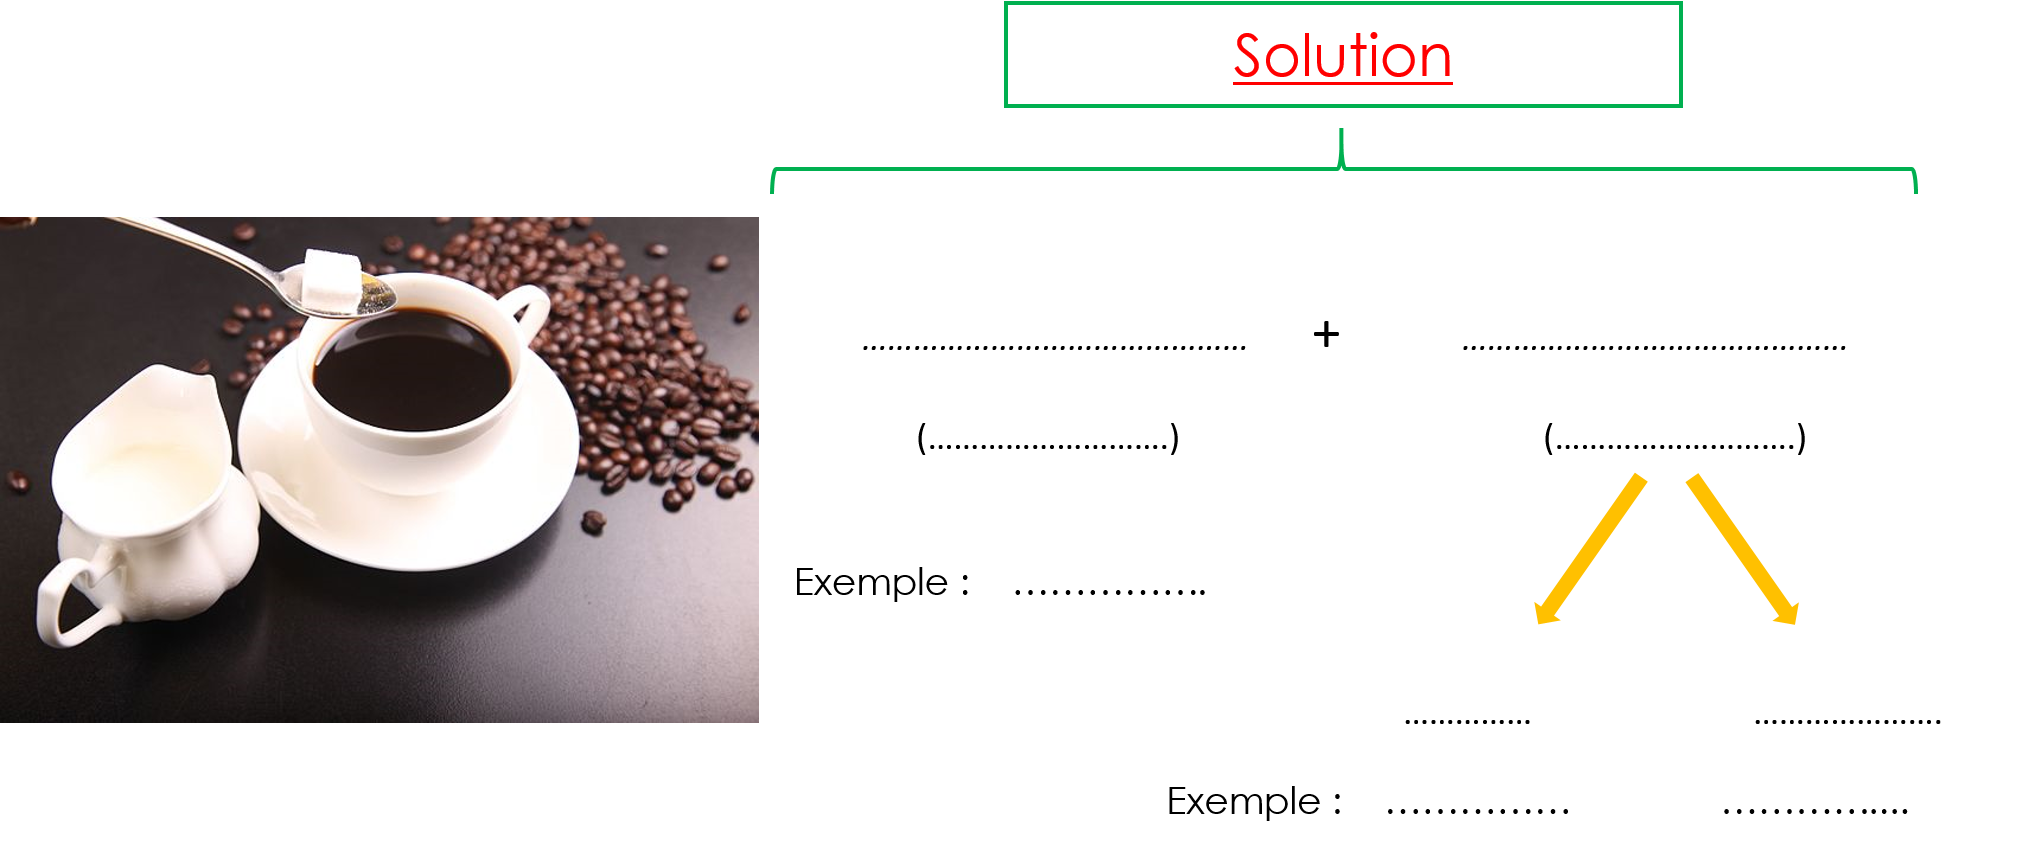
\includegraphics[width=\textwidth]{Images/Solution_def.png}
\end{center}
\end{tcolorbox}
Sur l'image de la tasse de café ci-dessus, qui jouent le rôle du solvant et des solutés ? Comment s'appelle la solution ?\\
\textit{Réponse :} \gap{........................................................................................................................}\\

\begin{Large}
    \ding{45}
\end{Large}\textbf{Exercice DOC : l'alcool dénaturé.}
\section{Concentration en masse et solubilité}
\subsection{Concentration en masse}
\begin{tcolorbox}[colback=green!5!white,colframe=green!75!black,title=\textbf{Définition}, upperbox=invisible]
La concentration en masse d’un soluté dans une 
solution est la masse de soluté dissous $m_{\text{soluté}}$ par rapport au volume de solution $V_{\text{solution}}$ :
\begin{equation*}
    C_m = \frac{m_{\text{soluté}}}{V_{\text{solution}}}
\end{equation*}
Elle est notée $C_m$ et elle s’exprime en gramme par litre (\textbf{g.L$^{-1}$}).
\end{tcolorbox}

\importantbox{
\begin{Large}
    \ding{43}
\end{Large}\textit{Voir activité 1 : Concentration en masse}
\begin{empheq}[box=\fbox]{equation*}
    C_m = \frac{m_{\text{soluté}}}{V_{\text{solution}}} \neq \rho = \frac{m_{\text{solution}}}{V_{\text{solution}}}
\end{empheq}
}
\begin{Large}
    \ding{45}
\end{Large}\textit{Exercices 14, 15, 25}\\

\textcolor{blue}{\textbf{Remarque :}} Peut-on ajouter une quantité infinie de soluté dans un solvant ? Non bien sûr, il existe une quantité maximale de soluté qu'on peut dissoudre dans un solvant : c'est la solubilité.
\subsection{Solubilité}
Comprendre la solubilité en vidéo : \url{https://www.youtube.com/watch?v=8bkfkRu_mbg}\\
\begin{Large}
    \faFlask
\end{Large} \textcolor{blue}{\textbf{Expérience :}} Dissolution de sel dans l'eau et dans l'huile.
\begin{tcolorbox}[colback=green!5!white,colframe=green!75!black,title=\textbf{Définition}, upperbox=invisible]
La solubilité, notée $s$, d'une espèce chimique est la masse maximale de cette espèce que l'on peut dissoudre dans $1$~L de solvant. Elle s'exprime en $\mathbf{g.L^{-1}}$.\\
Il s'agit d'une \textbf{concentration massique} !\\

La solubilité d'un soluté particulier dépend : 
\begin{center}
   1. de la température,\\
   2. du solvant utilisé.
\end{center}
\end{tcolorbox}

\section{Préparer des solutions aqueuses}

\subsection{Préparer par dissolution}
Le principe est de dissoudre une certaine masse de soluté (en général, il s'agit d'un solide) dans un volume précis d'eau afin d'obtenir une solution aqueuse de concentration en masse de soluté bien précise.

\begin{tcolorbox}[colback=red!5!white,colframe=red!75!black,title=\textbf{Protocole de préparation de la dissolution (résumé) : }, upperbox=invisible]
    \vspace{10cm}
\end{tcolorbox}


\begin{mdframed}[style=autreexo]
\textbf{\bsc{Exercice de cours} - Dissolution}\\
On souhaite préparer par dissolution 100 mL d’une solution aqueuse de concentration en masse de sulfate de cuivre égale à 15 g.L$^{-1}$. Calculer la masse de soluté à peser.\end{mdframed}
\gap{.......................................................................................................................................}
\newline
\gap{.......................................................................................................................................}\\
\begin{Large}
    \ding{45}
\end{Large}\textit{Exercice 18}

\subsection{Préparer par dilution}
Le principe est de prélever un certain volume d'une solution concentrée initiale appelée \textcolor{red}{solution mère} puis d'y ajouter de l'eau pour obtenir une solution moins concentrée appelée \textcolor{red}{solution fille} :
\begin{center}
    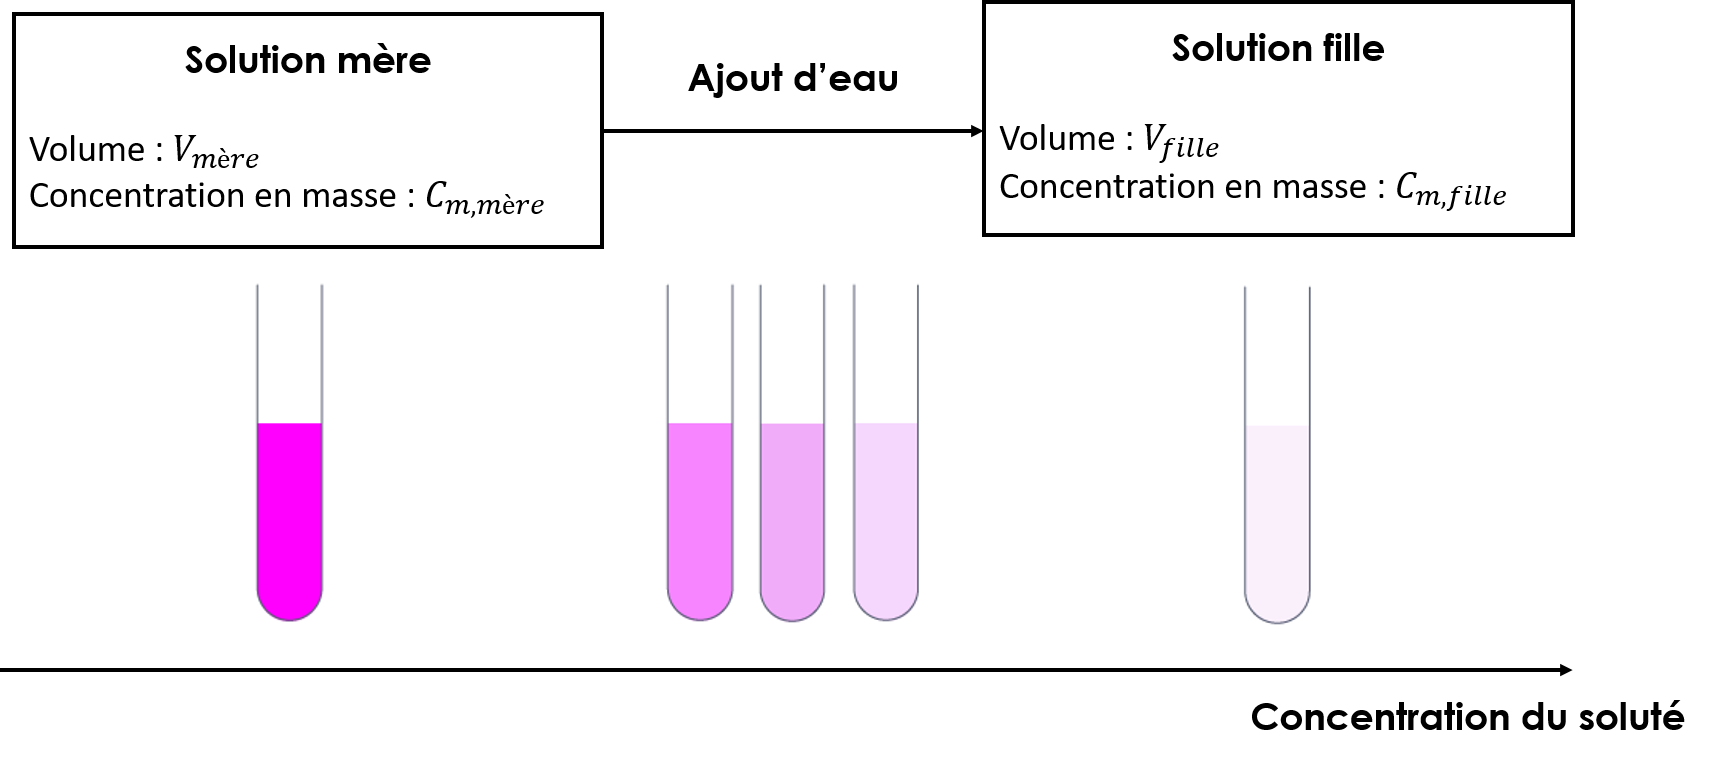
\includegraphics[scale=0.59]{Images/Dilution.png}
\end{center}
\begin{tcolorbox}[colback=red!5!white,colframe=red!75!black,title=\textbf{Propriété de la dilution : }, upperbox=invisible]
Au cours d'une dilution, la masse de soluté prélevée se conserve :
\begin{empheq}[box=\fbox]{align*}
    m_{\text{prélevée, mère}} &= m_{\text{soluté, fille}}\\
    C_{m,\text{mère}}V_{\text{prélevé}} &= C_{m,fille}V_{\text{fille}}
\end{empheq}
On peut dès lors définir le \textcolor{red}{facteur de dilution}, noté $F$ de la manière suivante :
\begin{equation*}
    F=\frac{C_{m,\text{mère}}}{C_{m,fille}} = \frac{V_{\text{fille}}}{V_{\text{prélevé}}}
\end{equation*}
\end{tcolorbox}
\begin{center}
    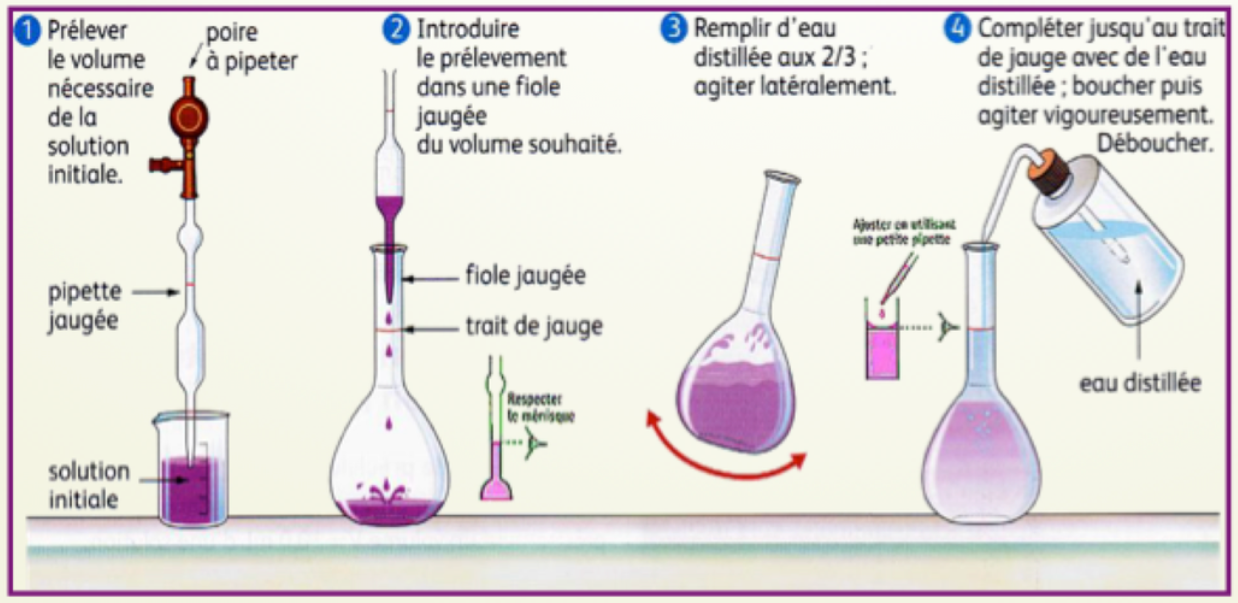
\includegraphics[scale=0.6]{Images/Protocole_dilution.png}
\end{center}

Avant de préparer une solution aqueuse par  dilution, il faut calculer le volume $V_{\text{mère}}$ de solution mère à 
prélever.\\

\begin{mdframed}[style=autreexo]
\textbf{\bsc{Exercice de cours} - Dilution}\\
On souhaite préparer par dilution 100 mL d’une solution aqueuse de concentration en masse de sulfate de cuivre égale à 15 g.L$^{-1}$ à partir d’une solution aqueuse de concentration en masse de sulfate de cuivre égale à 60 g.L$^{-1}$. Calculer le volume de solution mère à prélever. Calculer le facteur de dilution $F$.
\end{mdframed}

\gap{.......................................................................................................................................}
\newline
\gap{.......................................................................................................................................}
\newline
\gap{.......................................................................................................................................}
\newline
\gap{.......................................................................................................................................}\\

\begin{Large}
    \ding{45}
\end{Large}\textit{Exercices 16, 21}
\section{Détermination de la concentration en masse d'une solution}

\subsection{Echelle de teinte}
\begin{Large}
    \ding{43}
\end{Large}\textit{Voir TP : Préparer un médicament par dilution}\\
Partons de l'exemple suivant : on peut savoir si un verre de sirop dilué par de l'eau est plus ou moins concentré en sirop, simplement en regardant la couleur du mélange par rapport à la couleur du sirop sans eau. En faisant cela, on réalise sans le savoir une \textcolor{red}{échelle de teinte}. La solution diluée est appelée \textcolor{red}{solution étalon}.\\
En chimie, l'utilisation d'une échelle de teinte permet \textbf{d'encadrer la valeur d'une concentration en masse d'un soluté coloré}. Regardons la figure suivante :

\begin{center}
    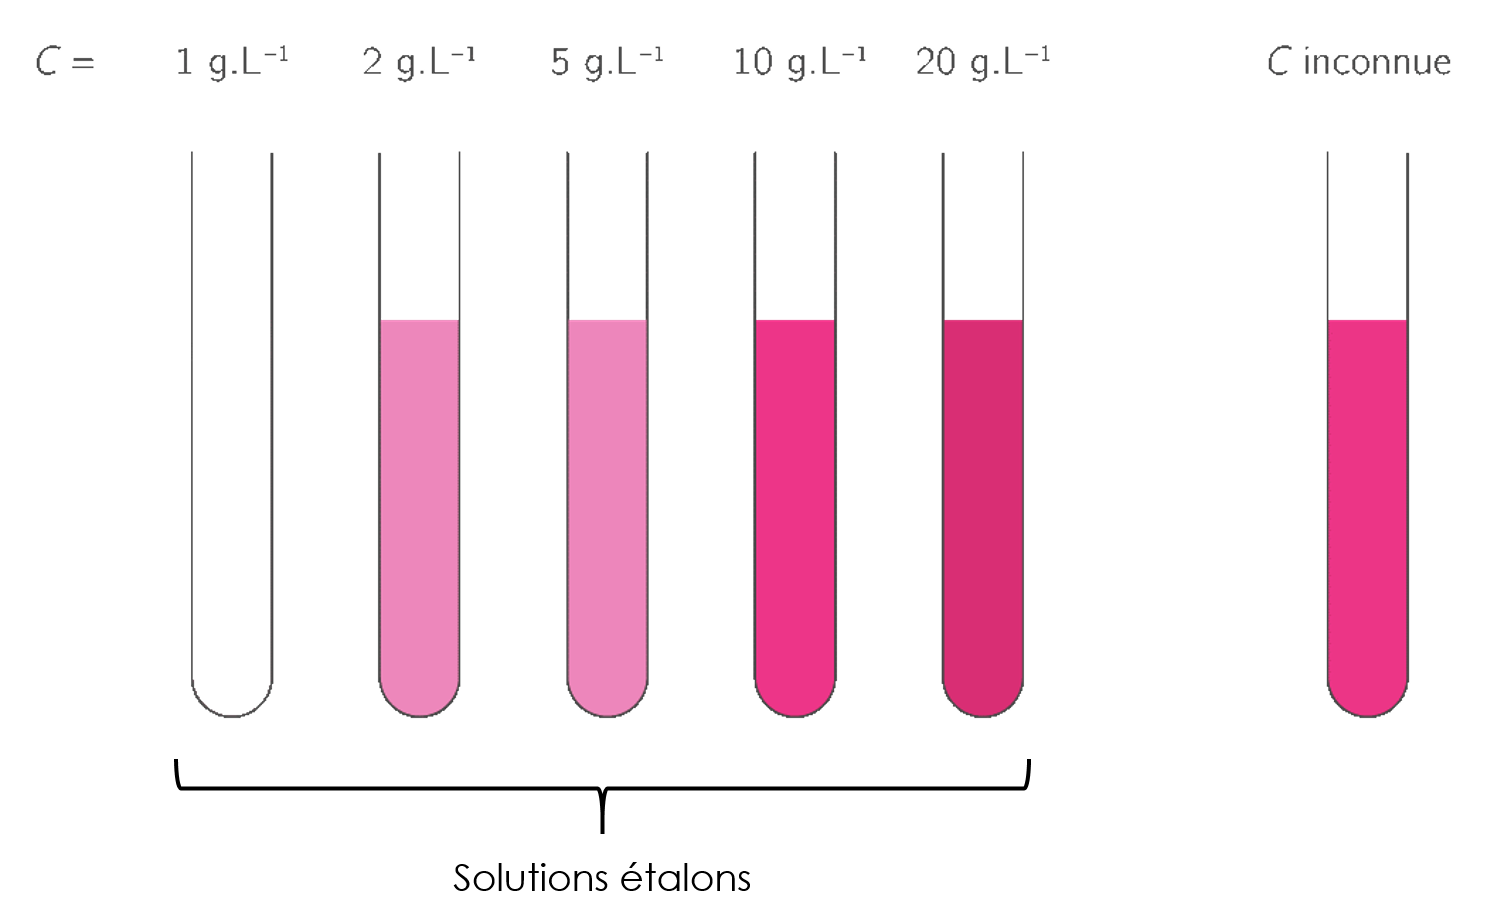
\includegraphics[scale=0.45]{Images/Echelle_teinte.png}
\end{center}

\begin{mdframed}[style=autreexo]
\textbf{\bsc{Exercice de cours} - Echelle de teinte}\\
Encadrer la concentration $C_{inconnue}$ en visualisant l'écchelle de teinte réalisée ci-dessus.
\end{mdframed}


\subsection{Par une courbe d'étalonnage}
\begin{Large}
    \ding{43}
\end{Large}\textit{Voir TP : Les sodas sont-ils très sucrés ?}\\
Une deuxième méthode plus précise consiste à réaliser une \textcolor{red}{courbe d'étalonnage} d'une grandeur physique ou chimique (par exemple : la masse volumique $\rho$, la conductivité $\sigma$, l'absorbance $A$ d'une solution, etc) à partir des solutions étalons.

\begin{center}
    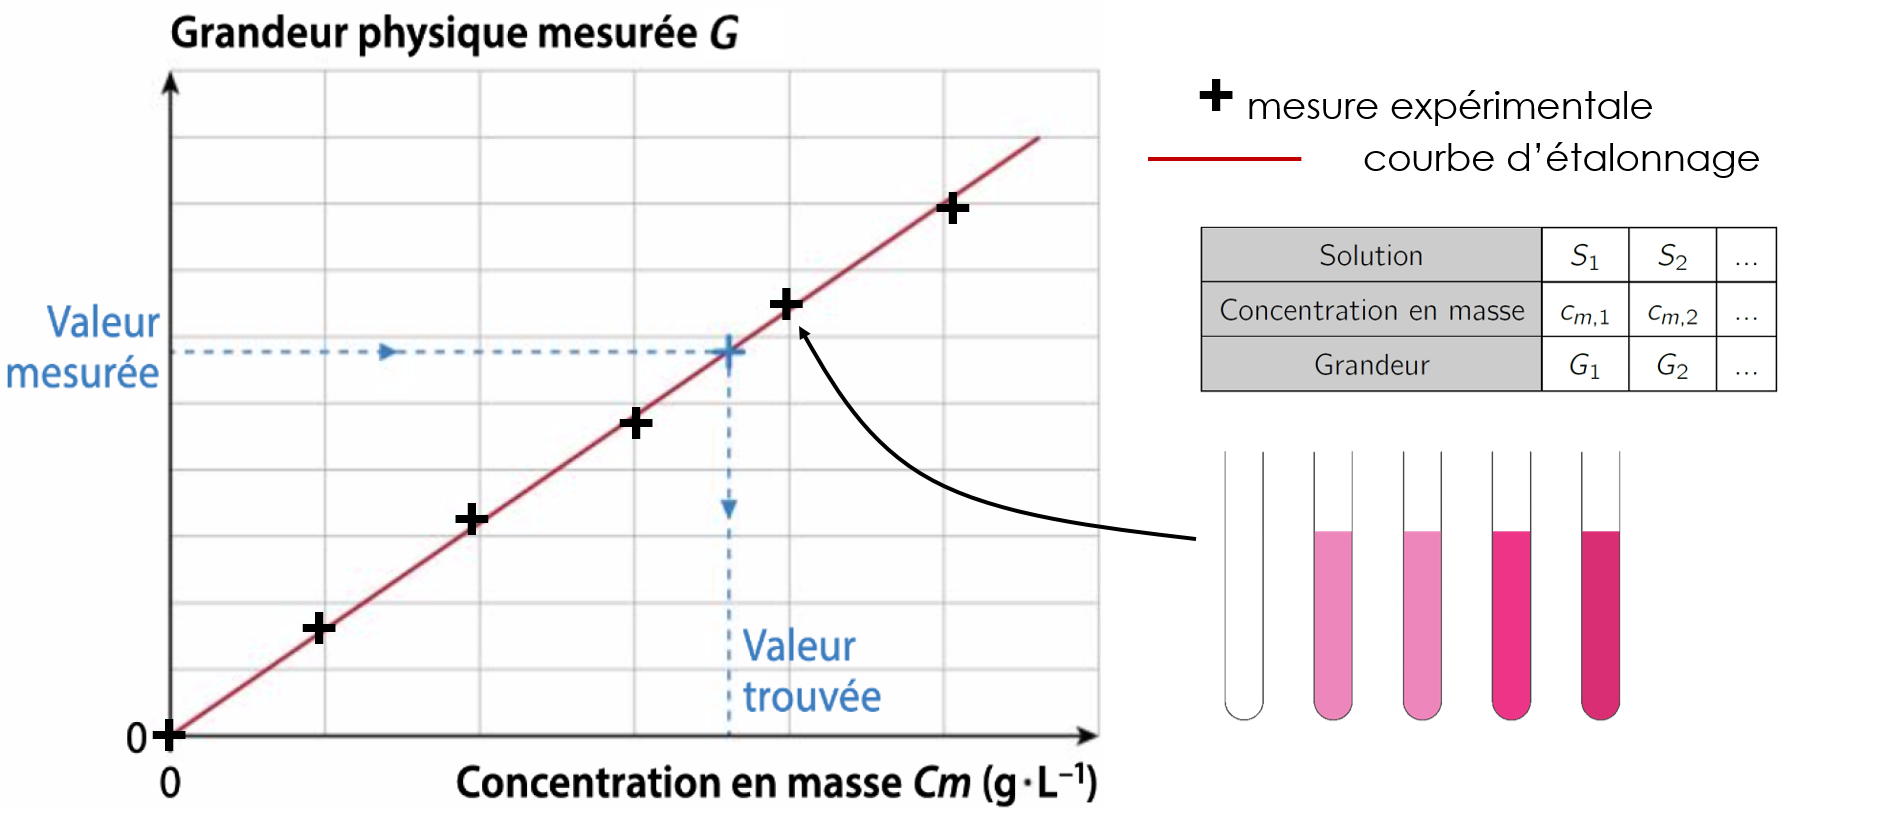
\includegraphics[scale=0.6]{Images/Courbe_etalonnage.png}
\end{center}

\begin{tcolorbox}[colback=red!5!white,colframe=red!75!black,title=\textbf{Protocole expérimental pour réaliser une courbe d'étalonnage: }, upperbox=invisible]
\begin{enumerate}
    \item Préparer une série de solutions étalons, c’est-à-dire des solutions obtenues à partir du même soluté que la solution de concentration inconnue et dont les concentrations en masse sont connues,
    \item Mesurer la valeur de la grandeur G pour chacune des solutions étalons,
    \item À partir des mesures précédentes, tracer la courbe représentant la grandeur $G$ en fonction de la concentration en masse $C_m$, appelée courbe d’étalonnage,
    \item Lorsque la grandeur $G$ est proportionnelle à concentration en masse $C_m$, la courbe d’étalonnage est une droite qui passe par l’origine,
    \item Mesurer la valeur de la grandeur $G$ pour la solution de concentration inconnue,
    \item Déterminer la concentration inconnue par lecture graphique sur la courbe d’étalonnage.
\end{enumerate}
\end{tcolorbox}
  %\renewcommand{\thesubsection}{\textcolor{red}{\Roman{section}.\arabic{subsection}}}
\renewcommand{\thesubsubsection}{\textcolor{red}{\Roman{section}.\arabic{subsection}.\alph{subsubsection}}}

\setcounter{section}{0}
\sndEnTeteCoursDeux

\begin{mdframed}[style=titr, leftmargin=60pt, rightmargin=60pt, innertopmargin=7pt, innerbottommargin=7pt, innerrightmargin=8pt, innerleftmargin=8pt]

\begin{center}
\large{\textbf{Chapitre 2 : Les solutions aqueuses}}
\end{center}
\end{mdframed}
Dans ce chapitre, nous nous intéressons à un type de mélanges homogènes en particulier : les solutions aqueuses. 

\begin{tcolorbox}[colback=blue!5!white,colframe=blue!75!black,title=Mots clés du chapitre :]
Solution, solvant, soluté, solubilité, dissolution, dilution, échelle de teinte, courbe d'étalonnage. 
\end{tcolorbox}


\section{Composition d'une solution}
\begin{Large}
    \ding{43}
\end{Large}\textit{Voir activité 1 : Concentration en masse}
\begin{tcolorbox}[colback=green!5!white,colframe=green!75!black,title=\textbf{Solution, solvant, soluté}]
\begin{center}
    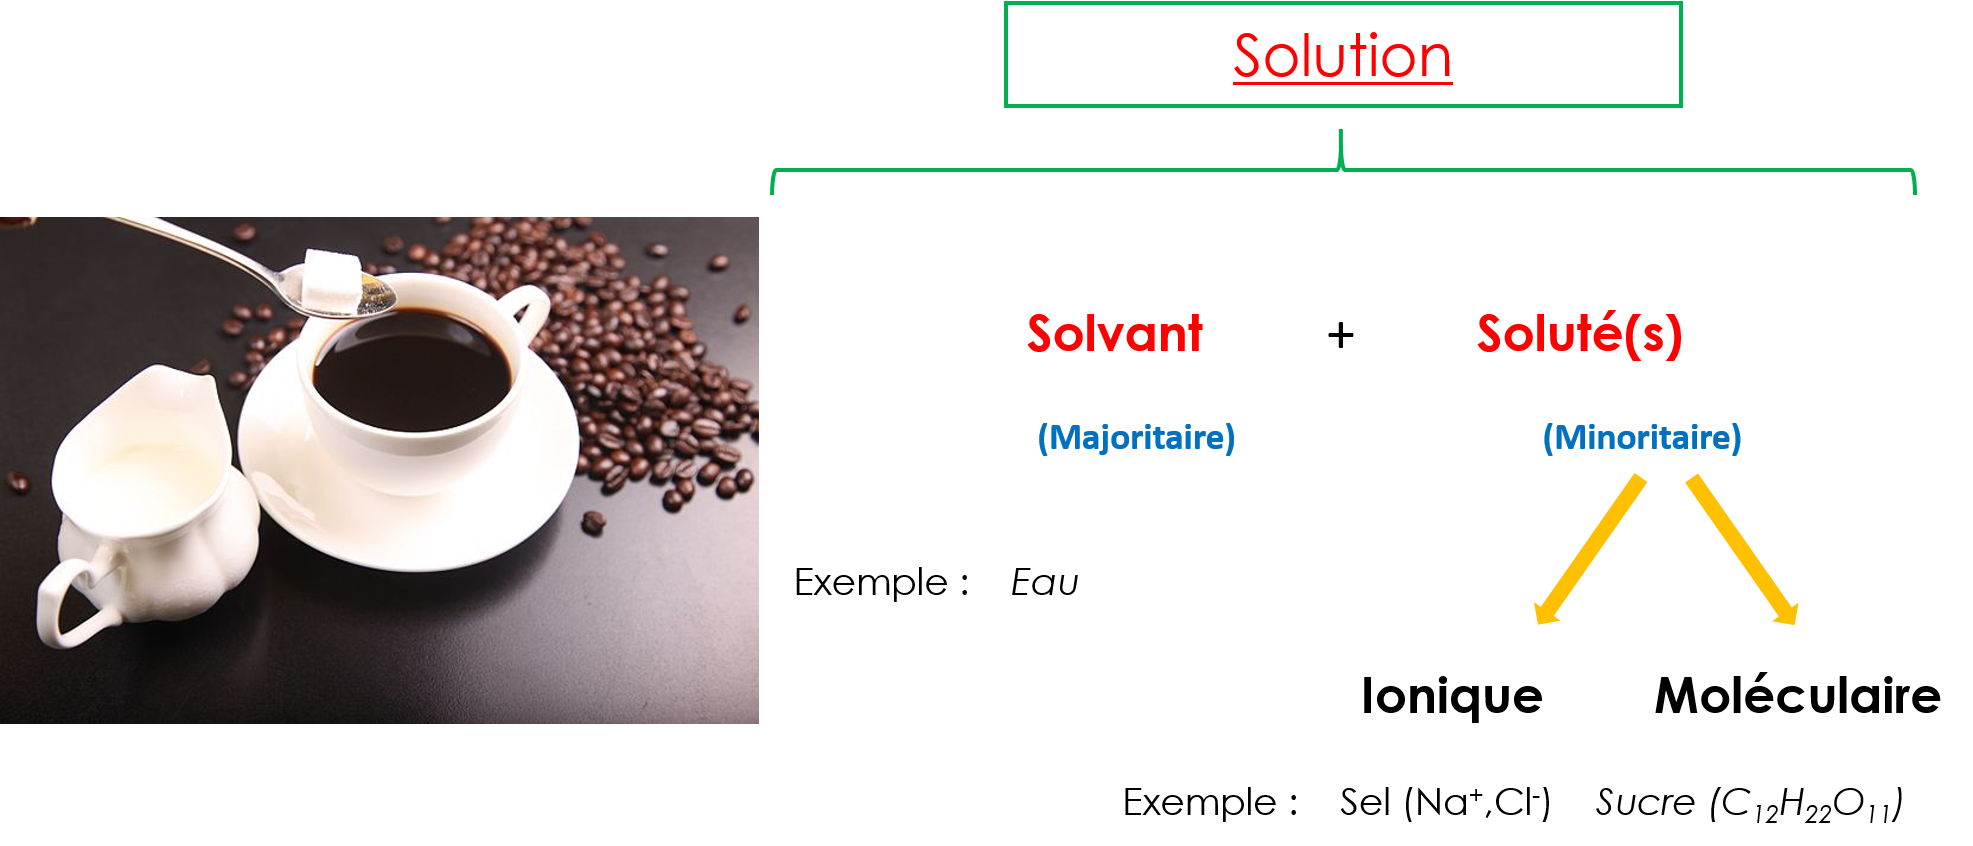
\includegraphics[width=\textwidth]{Images/Solution_def_corr.png}
\end{center}
\end{tcolorbox}
Sur l'image de la tasse de café ci-dessus, qui jouent le rôle du solvant et des solutés ? Comment s'appelle la solution ?\\
\textit{Réponse : Le solvant est l'eau, un soluté possible est le sucre.}

\begin{Large}
    \ding{45}
\end{Large}\textbf{Exercice DOC : l'alcool dénaturé.}

\section{Concentration en masse et solubilité}
\subsection{Concentration en masse}
\begin{tcolorbox}[colback=green!5!white,colframe=green!75!black,title=\textbf{Définition}]
La concentration en masse d’un soluté dans une 
solution est la masse de soluté dissous $m_{\text{soluté}}$ par rapport au volume de solution $V_{\text{solution}}$ :
\begin{equation*}
    C_m = \frac{m_{\text{soluté}}}{V_{\text{solution}}}
\end{equation*}
Elle est notée $C_m$ et elle s’exprime en gramme par litre (\textbf{g.L$^{-1}$}).
\end{tcolorbox}

\importantbox{
\begin{Large}
    \ding{43}
\end{Large}\textit{Voir activité 1 : Concentration en masse}
\begin{empheq}[box=\fbox]{equation*}
    C_m = \frac{m_{\text{soluté}}}{V_{\text{solution}}} \neq \rho = \frac{m_{\text{solution}}}{V_{\text{solution}}}
\end{empheq}
}
\begin{Large}
    \ding{45}
\end{Large}\textit{Exercices 14, 15, 25}\\

\textcolor{blue}{\textbf{Remarque :}} Peut-on ajouter une quantité infinie de soluté dans un solvant ? Non bien sûr, il existe une quantité maximale de soluté qu'on peut dissoudre dans un solvant : c'est la solubilité.
\subsection{Solubilité}
Comprendre la solubilité en vidéo : \url{https://www.youtube.com/watch?v=8bkfkRu_mbg}\\
\begin{Large}
    \faFlask
\end{Large} \textcolor{blue}{\textbf{Expérience :}} Dissolution de sel dans l'eau et dans l'huile.
\begin{tcolorbox}[colback=green!5!white,colframe=green!75!black,title=\textbf{Définition}]
La solubilité, notée $s$, d'une espèce chimique est la masse maximale de cette espèce que l'on peut dissoudre dans $1$~L de solvant. Elle s'exprime en $\mathbf{g.L^{-1}}$.\\
Il s'agit d'une \textbf{concentration massique} !\\

La solubilité d'un soluté particulier dépend : 
\begin{center}
   1. de la température,\\
   2. du solvant utilisé.
\end{center}
\end{tcolorbox}

\section{Préparer des solutions aqueuses}

\subsection{Préparer par dissolution}
Le principe est de dissoudre une certaine masse de soluté (en général, il s'agit d'un solide) dans un volume précis d'eau afin d'obtenir une solution aqueuse de concentration en masse de soluté bien précise.
\begin{center}
    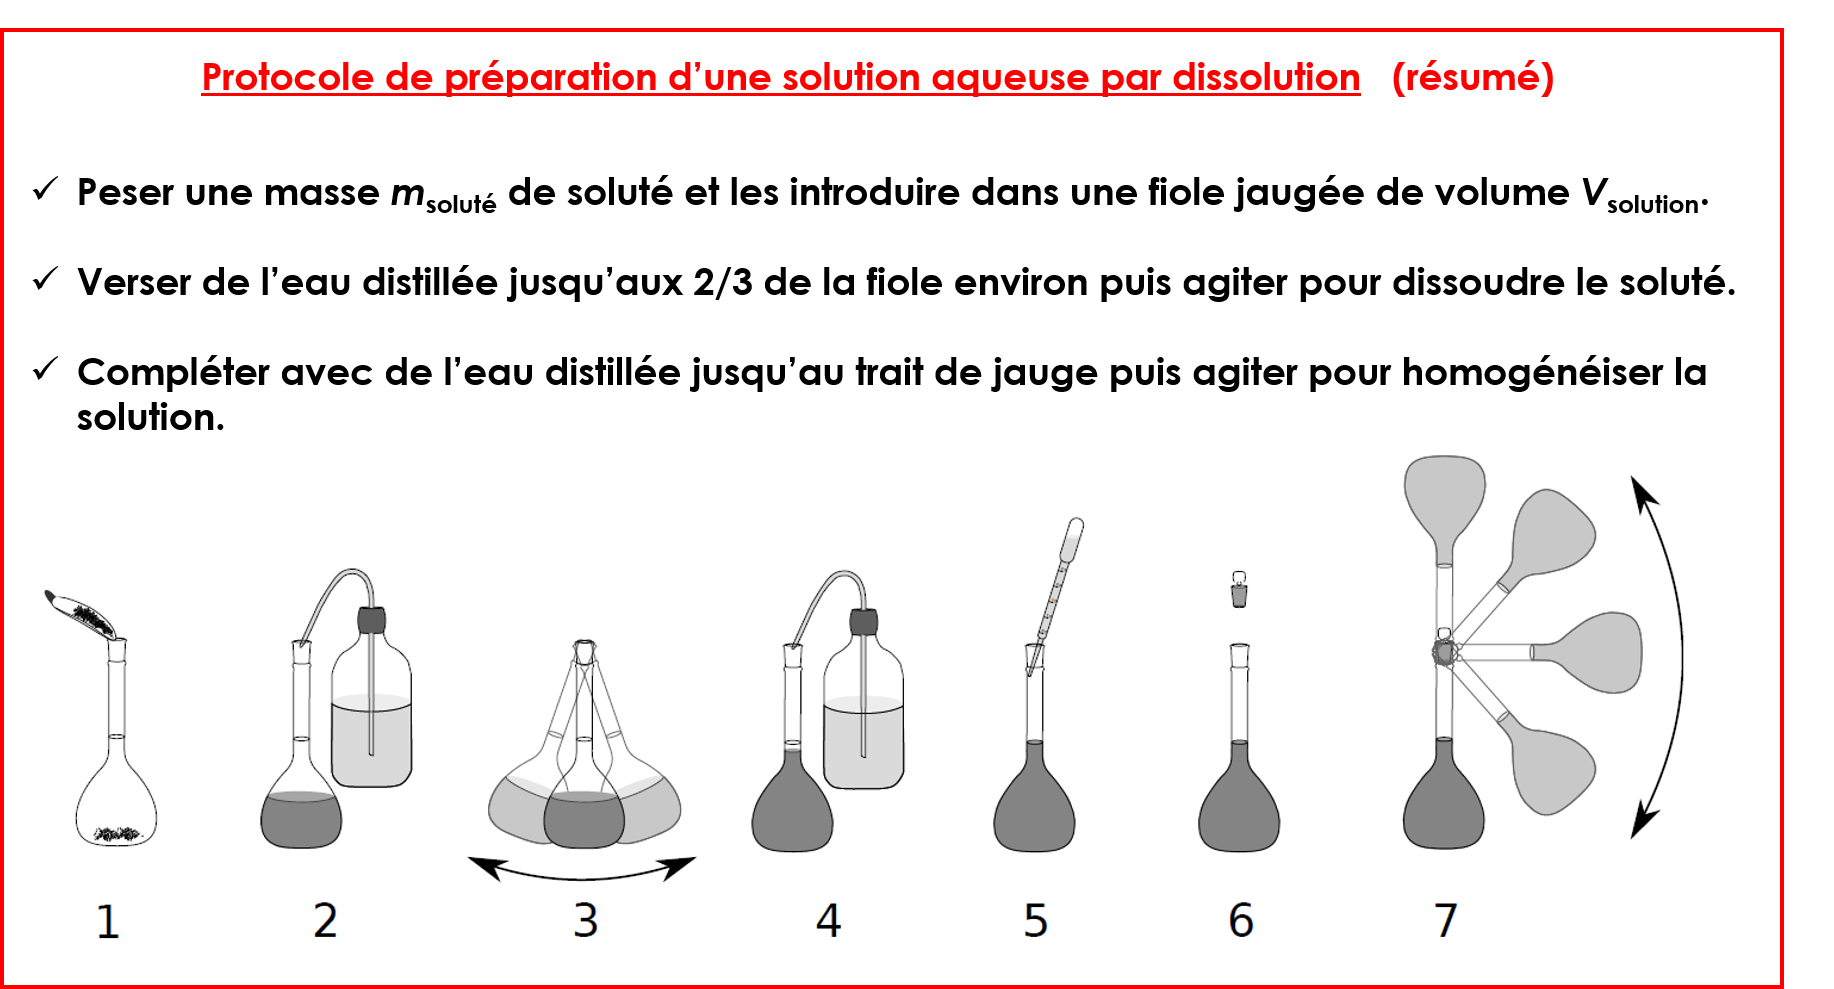
\includegraphics[scale=0.59]{Images/Dissolution.png}
\end{center}

\begin{mdframed}[style=autreexo]
\textbf{\bsc{Exercice de cours} - Dissolution}\\
On souhaite préparer par dissolution 100 mL d’une solution aqueuse de concentration en masse de sulfate de cuivre égale à 15 g.L$^{-1}$. Calculer la masse de soluté à peser.\end{mdframed}
\textit{Réponse : On sait que $C_m = \frac{m_{\text{soluté}}}{V_{solution}}$ donc $m_{\text{soluté}}=C_m\times V_{solution} =15~\text{g.L$^{-1}$}\times 0,100~\text{L} = 1,5$~g}.\\

\begin{Large}
    \ding{45}
\end{Large}\textit{Exercice 18}

\subsection{Préparer par dilution}
Le principe est de prélever un certain volume d'une solution concentrée initiale appelée \textcolor{red}{solution mère} puis d'y ajouter de l'eau pour obtenir une solution moins concentrée appelée \textcolor{red}{solution fille} :
\begin{center}
    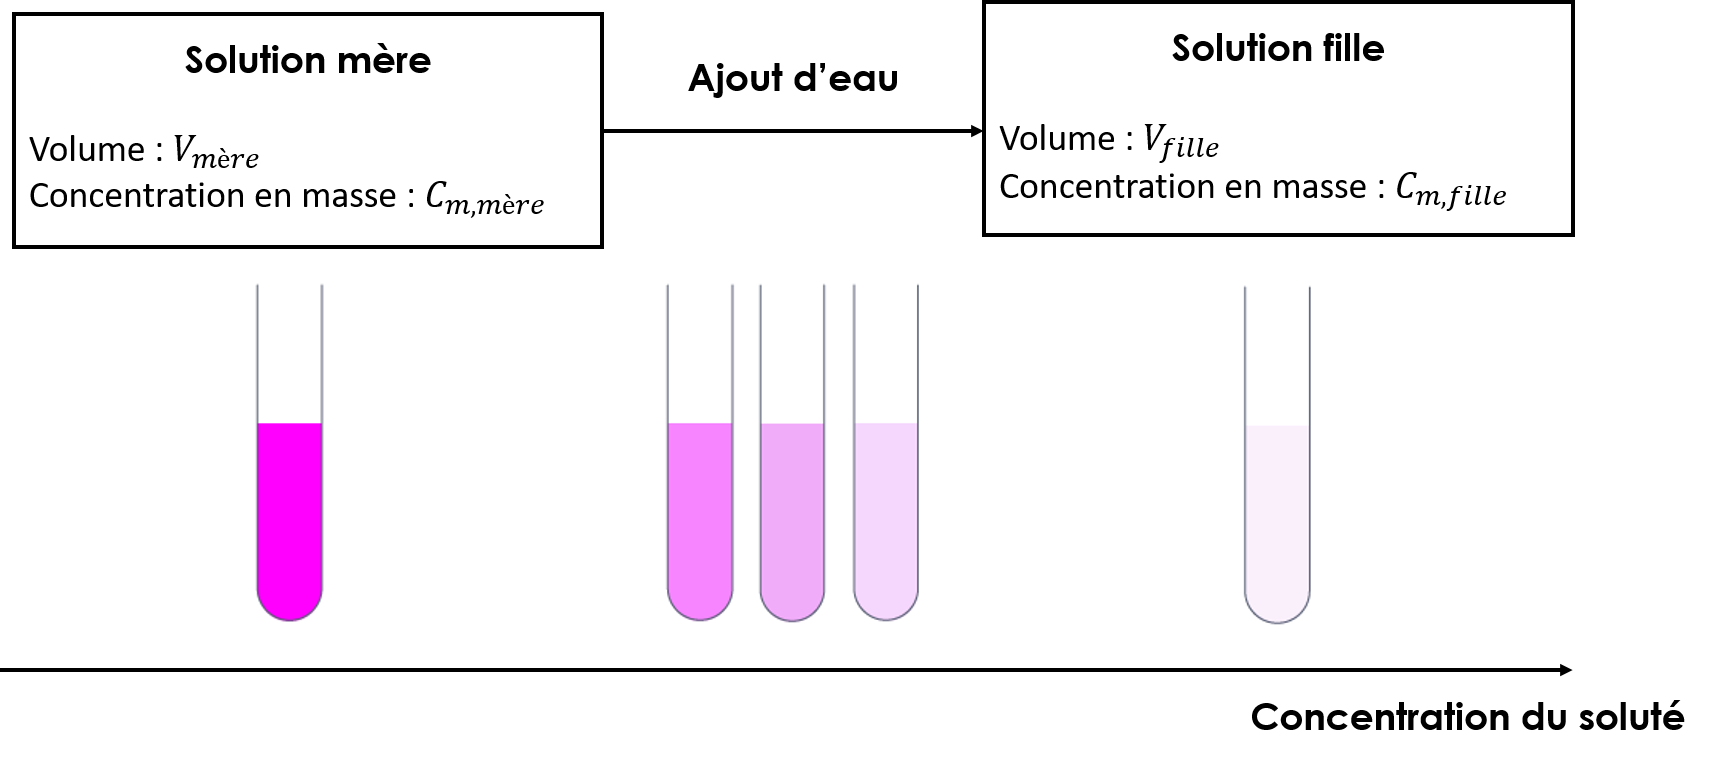
\includegraphics[scale=0.59]{Images/Dilution.png}
\end{center}
\begin{tcolorbox}[colback=red!5!white,colframe=red!75!black,title=\textbf{Propriété de la dilution : }]
Au cours d'une dilution, la masse de soluté prélevée se conserve :
\begin{empheq}[box=\fbox]{align*}
    m_{\text{prélevée, mère}} &= m_{\text{soluté, fille}}\\
    C_{m,\text{mère}}V_{\text{prélevé}} &= C_{m,fille}V_{\text{fille}}
\end{empheq}
On peut dès lors définir le \textcolor{red}{facteur de dilution}, noté $F$ de la manière suivante :
\begin{equation*}
    F=\frac{C_{m,\text{mère}}}{C_{m,fille}} = \frac{V_{\text{fille}}}{V_{\text{prélevé}}}
\end{equation*}
\end{tcolorbox}
\begin{center}
    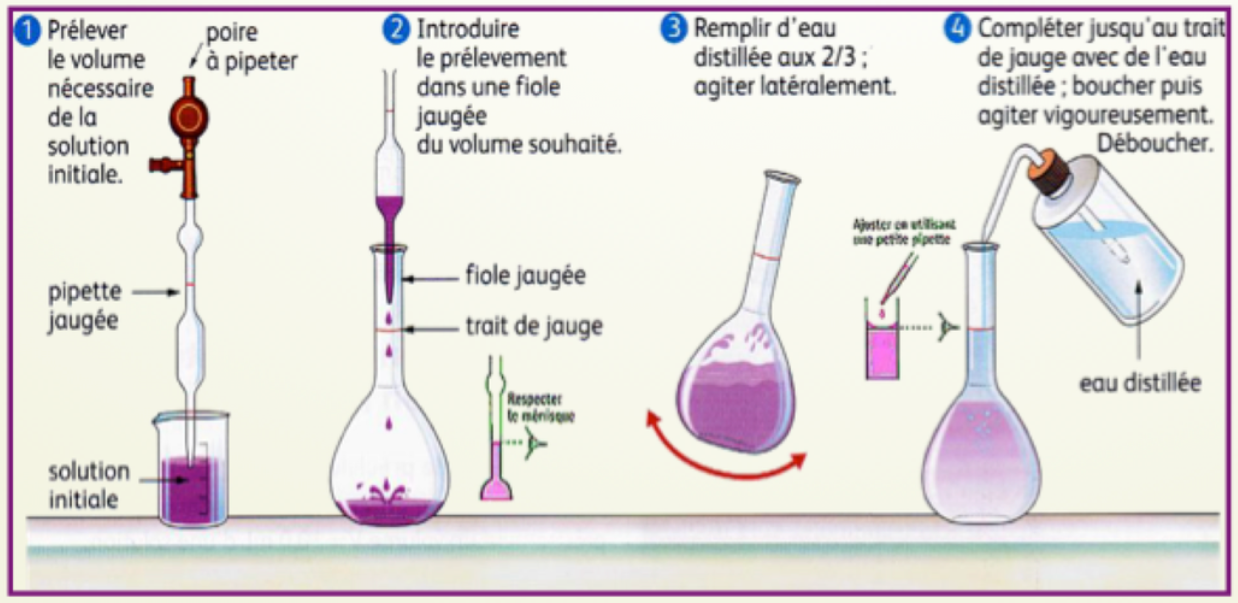
\includegraphics[scale=0.6]{Images/Protocole_dilution.png}
\end{center}

Avant de préparer une solution aqueuse par  dilution, il faut calculer le volume $V_{\text{mère}}$ de solution mère à 
prélever.\\

\begin{mdframed}[style=autreexo]
\textbf{\bsc{Exercice de cours} - Dilution}\\
On souhaite préparer par dilution 100 mL d’une solution aqueuse de concentration en masse de sulfate de cuivre égale à 15 g.L$^{-1}$ à partir d’une solution aqueuse de concentration en masse de sulfate de cuivre égale à 60 g.L$^{-1}$. Calculer le volume de solution mère à prélever. Calculer le facteur de dilution $F$.
\end{mdframed}
\textit{Réponse : On utilise la conservation de la masse de soluté : 
\begin{equation*}
    C_{m,\text{mère}}V_{\text{prélevé}} = C_{m,fille}V_{\text{fille}}
\end{equation*}
avec $V_{\text{fille}}=100$~mL, $C_{m,\text{mère}}=60$~g.L$^{-1}$ et $C_{m,\text{fille}}=15$~g.L$^{-1}$. On en déduit :
\begin{equation*}
    V_{\text{prélevé}}=\frac{C_{m,fille}V_{\text{fille}}}{C_{m,\text{mère}}}=\frac{15~\text{g.L$^{-1}$}\times100~\text{mL}}{60~\text{g.L$^{-1}$}}=25~\text{mL}
\end{equation*}
On en déduit $F=\frac{V_{fille}}{V_{\text{prélevé}}}=\frac{100~\text{mL}}{25~\text{mL}}=4$}.


\begin{Large}
    \ding{45}
\end{Large}\textit{Exercices 16, 21}
\section{Détermination de la concentration en masse d'une solution}

\subsection{Echelle de teinte}
\begin{Large}
    \ding{43}
\end{Large}\textit{Voir TP : Préparer un médicament par dilution}\\
Partons de l'exemple suivant : on peut savoir si un verre de sirop dilué par de l'eau est plus ou moins concentré en sirop, simplement en regardant la couleur du mélange par rapport à la couleur du sirop sans eau. En faisant cela, on réalise sans le savoir une \textcolor{red}{échelle de teinte}. La solution diluée est appelée \textcolor{red}{solution étalon}.\\
En chimie, l'utilisation d'une échelle de teinte permet \textbf{d'encadrer la valeur d'une concentration en masse d'un soluté coloré}. Regardons la figure suivante :

\begin{center}
    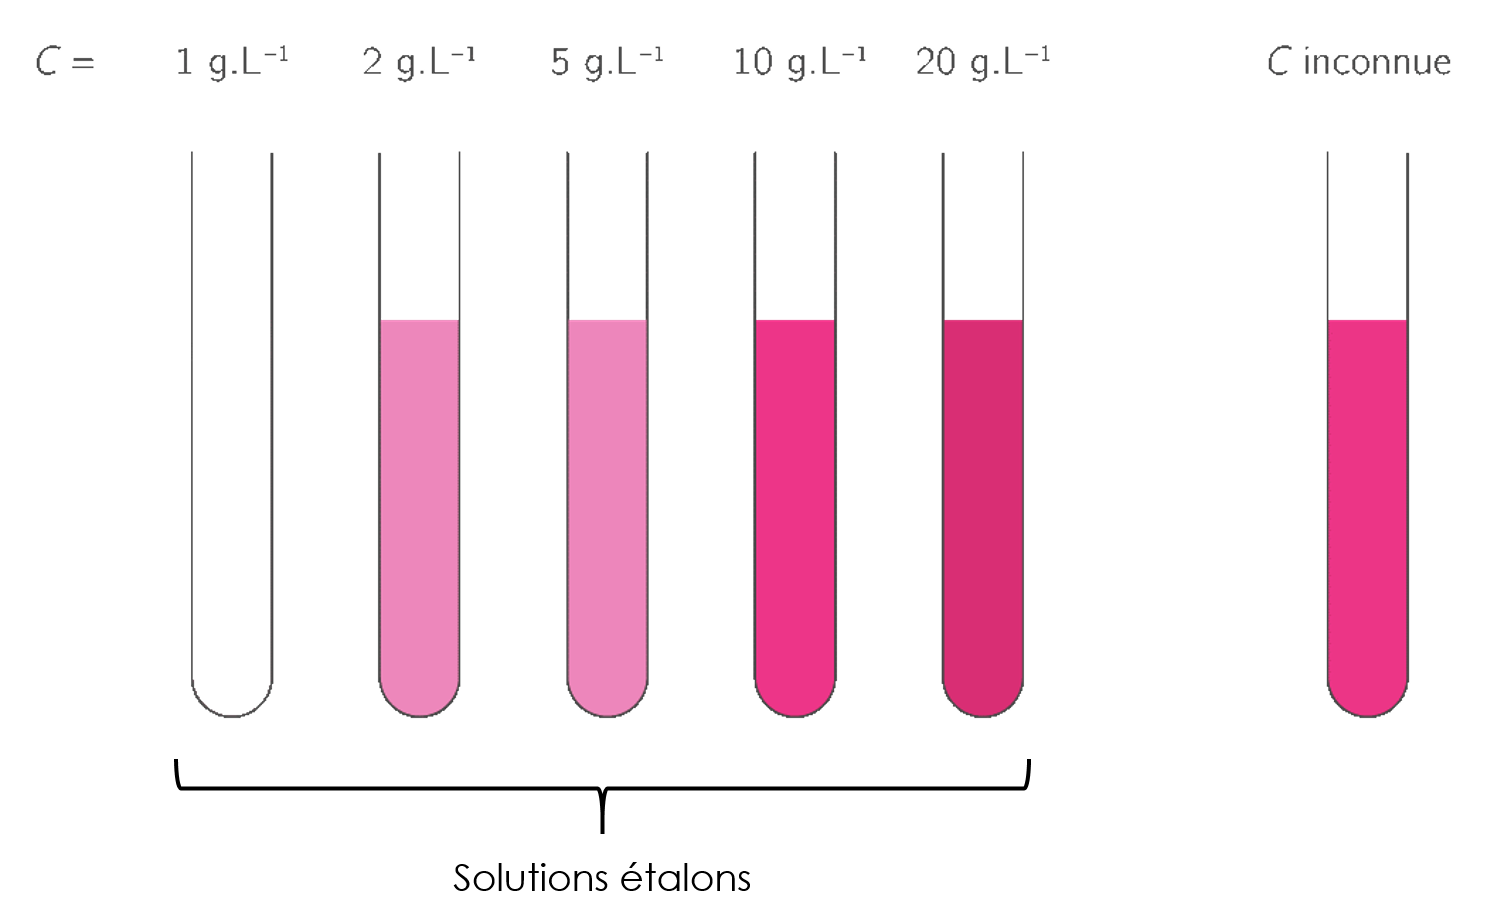
\includegraphics[scale=0.45]{Images/Echelle_teinte.png}
\end{center}

\begin{mdframed}[style=autreexo]
\textbf{\bsc{Exercice de cours} - Echelle de teinte}\\
Encadrer la concentration $C_{inconnue}$ en visualisant l'écchelle de teinte réalisée ci-dessus.
\end{mdframed}
\textit{Réponse : On peut voir que la teinte de la concentration inconnue est plus foncée que la teinte de la solution étalon à 5~g.L$^{-1}$ mais plus claire que celle à 10~g.L$^{-1}$. On peut donc encadrer la concentration de la solution inconnue : $5~g.L^{-1}<C_{inconnue}<10~g.L^{-1}$} 


\subsection{Par une courbe d'étalonnage}
\begin{Large}
    \ding{43}
\end{Large}\textit{Voir TP : Les sodas sont-ils très sucrés ?}\\
Une deuxième méthode plus précise consiste à réaliser une \textcolor{red}{courbe d'étalonnage} d'une grandeur physique ou chimique (par exemple : la masse volumique $\rho$, la conductivité $\sigma$, l'absorbance $A$ d'une solution, etc) à partir des solutions étalons.

\begin{center}
    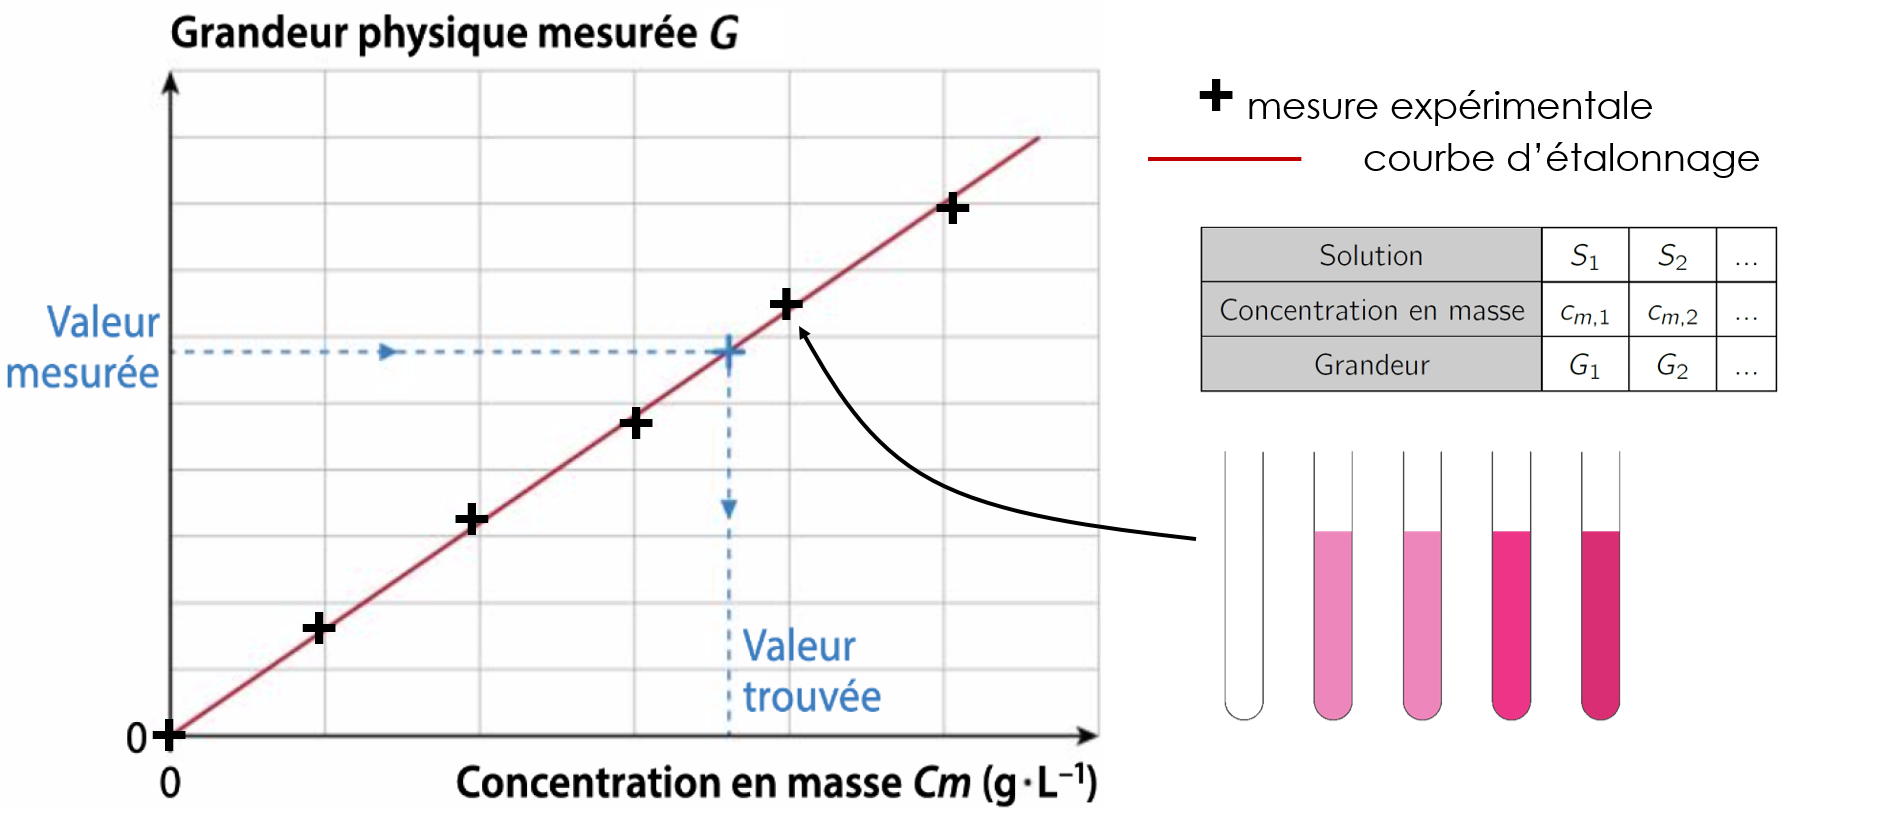
\includegraphics[scale=0.6]{Images/Courbe_etalonnage.png}
\end{center}

\begin{tcolorbox}[colback=red!5!white,colframe=red!75!black,title=\textbf{Protocole expérimental pour réaliser une courbe d'étalonnage: }]
\begin{enumerate}
    \item Préparer une série de solutions étalons, c’est-à-dire des solutions obtenues à partir du même soluté que la solution de concentration inconnue et dont les concentrations en masse sont connues,
    \item Mesurer la valeur de la grandeur G pour chacune des solutions étalons,
    \item À partir des mesures précédentes, tracer la courbe représentant la grandeur $G$ en fonction de la concentration en masse $C_m$, appelée courbe d’étalonnage,
    \item Lorsque la grandeur $G$ est proportionnelle à concentration en masse $C_m$, la courbe d’étalonnage est une droite qui passe par l’origine,
    \item Mesurer la valeur de la grandeur $G$ pour la solution de concentration inconnue,
    \item Déterminer la concentration inconnue par lecture graphique sur la courbe d’étalonnage.
\end{enumerate}
\end{tcolorbox}

  %%%%%%%%%% Exercices %%%%%%%%
  %\renewcommand{\thesubsection}{\textcolor{red}{\Roman{section}.\arabic{subsection}}}
\renewcommand{\thesubsubsection}{\textcolor{red}{\Roman{section}.\arabic{subsection}.\alph{subsubsection}}}

\setcounter{section}{0}
\sndEnTeteExerciceDeux

\begin{center}
\begin{mdframed}[style=titr, leftmargin=60pt, rightmargin=60pt, innertopmargin=7pt, innerbottommargin=7pt, innerrightmargin=8pt, innerleftmargin=8pt]

\begin{center}
\large{\textbf{Feuille d'exercices du Chapitre 2}}
\end{center}

\end{mdframed}
\end{center}

\section{Pour commencer}
\begin{mdframed}[style=autreexo]
\textbf{\bsc{Exercice 1} - Entoure la bonne réponse} 5min chrono !\\
\begin{enumerate}
    \item \textbf{Le sang est un liquide dont l'eau est :}
\begin{align*}
    a.& \text{ le soluté} & b.& \text{ le solvant} & c.& \text{ la solution}
\end{align*}
    \item \textbf{La concentration en masse d'une solution est le quotient de la masse du soluté par le volume de :}
    \begin{align*}
        a.& \text{ solvant} & b.& \text{ soluté} & c.& \text{ solution}
    \end{align*}
    \item \textbf{L'unité usuelle de la concentration en masse est :}
    \begin{align*}
        a.& \text{ le g.L$^{-1}$} & b.& \text{ le g.L} & c.& \text{  le L.g$^{-1}$}
    \end{align*}
    \item \textbf{Pour réaliser avec précision un volume V=50,0~mL d'ammoniac, il faut utiliser : }
    \begin{align*}
        a.& \text{un erlenmeyer} & b.& \text{ un bécher} & c.& \text{  une fiole jaugée}
    \end{align*}
    \item \textbf{Un échantillon de 10g d'aspirine est dissous dans 1,0L d'eau. La concentration en masse d'aspirine dans la solution acqueuse est :}
    \begin{align*}
        a.& \text{ 10 g.L$^{-1}$} & b.& \text{ 0,10 g.L$^{-1}$} & c.& \text{  1,0 g.L$^{-1}$}
    \end{align*}
    \item \textbf{La teinte d'un sirop de menthe est plus foncée que les teintes d'une gamme étalon dont les concentrations en masse sont comprises entre 1,0~mg.L$^{-1}$ et 10~mg.L$^{-1}$. La concentration en masse $c_m$ du sirop est :}
    \begin{align*}
        a.& \text{ $c_m$ < 1,0~mg.L$^{-1}$} & b.& \text{ 1,0~mg.L$^{-1}$ < $c_m$ < 10~mg.L$^{-1}$} & c.& \text{  $c_m$ > 10~mg.L$^{-1}$}
    \end{align*}
\end{enumerate}
\end{mdframed}

\begin{center}
    \includegraphics[scale=0.6]{Images/Exo_Doc.png}
\end{center}


\section{Pour s'entrainer}

\begin{center}
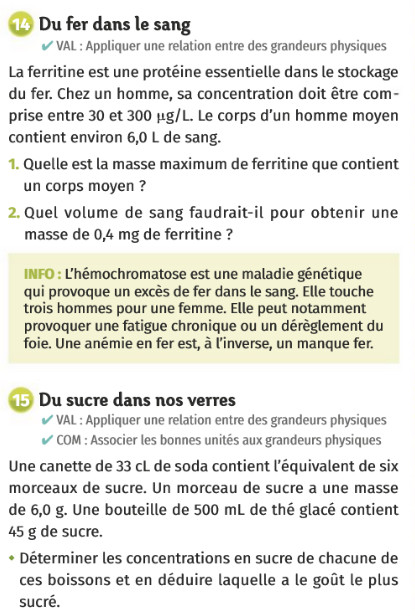
\includegraphics[scale=1.1]{Images/Ex_14.png}
\vspace{1cm}
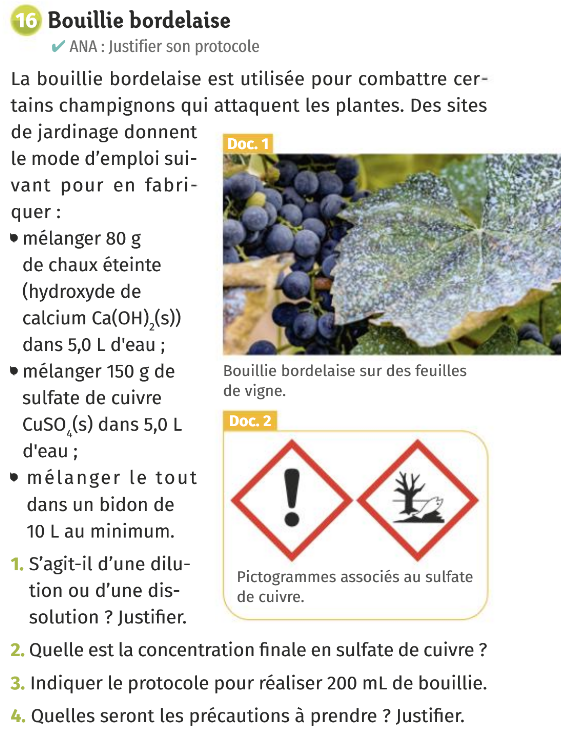
\includegraphics[scale=0.9]{Images/Ex_16.png}
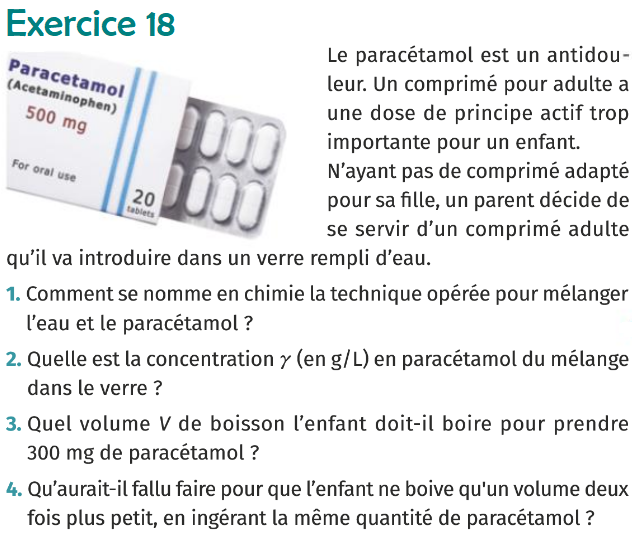
\includegraphics[scale=0.9]{Images/Exo_paracetamol.PNG}
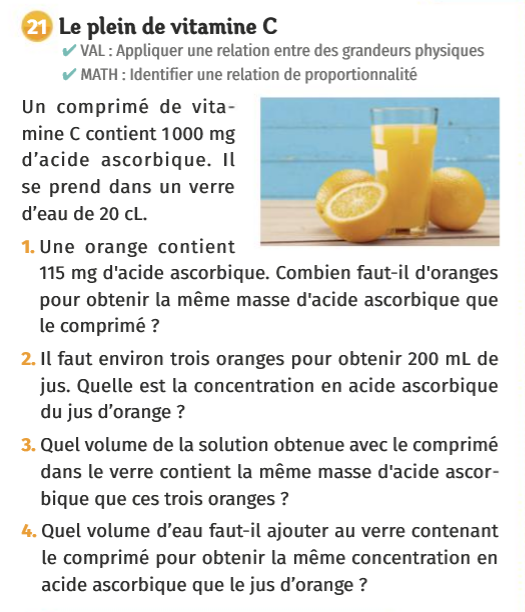
\includegraphics[scale=1.5]{Images/Ex_21.png}
\end{center}
\newpage
\begin{center}
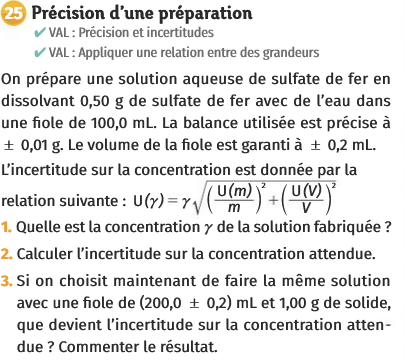
\includegraphics[scale=2]{Images/Ex_25.png}
\end{center}

\section{Pour aller plus loin}
\begin{center}
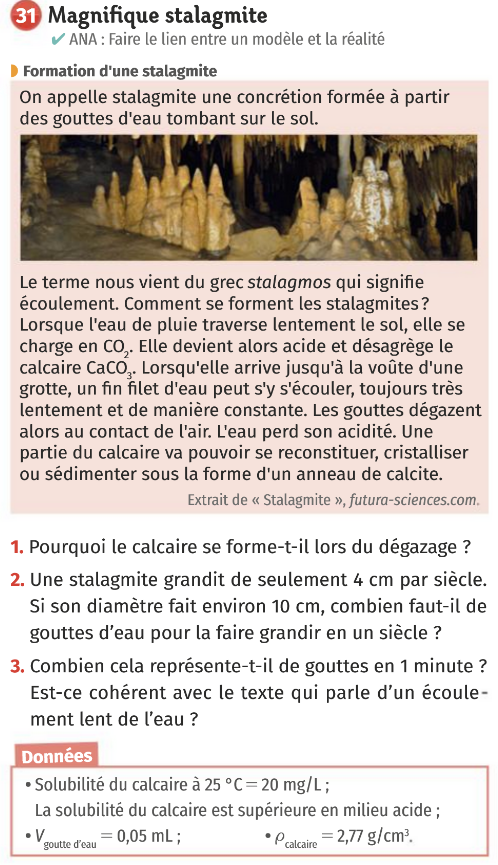
\includegraphics[scale=1.5]{Images/Ex_31.png}
\end{center}
\newpage
\begin{center}
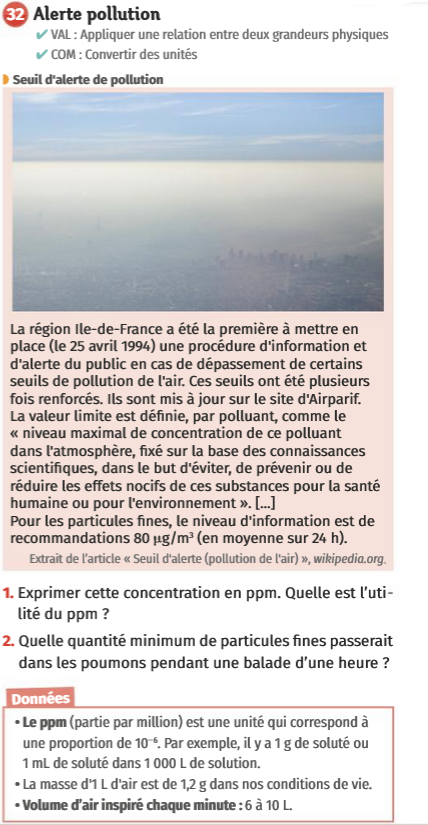
\includegraphics[scale=1.5]{Images/Ex_32.png}
\end{center}

  %%%%%%%%%% Activités %%%%%%%%
  %\modeCorrection

\renewcommand{\thesubsection}{\textcolor{red}{\Roman{section}.\arabic{subsection}}}
\renewcommand{\thesubsubsection}{\textcolor{red}{\Roman{section}.\arabic{subsection}.\alph{subsubsection}}}

\setcounter{section}{0}
\setcounter{document}{0}
\sndEnTeteActDeux

\begin{center}
\begin{mdframed}[style=titr, leftmargin=60pt, rightmargin=60pt, innertopmargin=7pt, innerbottommargin=7pt, innerrightmargin=8pt, innerleftmargin=8pt]

\begin{center}
\large{\textbf{Activité documentaire : Concentration en masse et masse volumique d'une solution acqueuse.}}
\end{center}

\end{mdframed}
\end{center}

\begin{tcolorbox}[colback=orange!5!white,colframe=orange!75!black,title= Contexte de l'activité]
Consommées en excès, certaines boissons peuvent être dangereuses pour la santé à cause de leur teneur en sucre. Quelle grandeur permet d’identifier, parmi plusieurs boissons, la boisson la plus sucrée ?
\end{tcolorbox}
\begin{tcolorbox}[colback=blue!5!white,colframe=blue!75!black,title=Objectifs :]
\begin{itemize}
    \item Identifier le solvant et le(s) soluté(s) d’une solution,
    \item Déterminer la valeur de la concentration en masse d’un soluté dans une solution à partir de résultats expérimentaux,
    \item Distinguer la masse volumique d’une solution et la concentration en masse d’un soluté dans une solution.
\end{itemize}
\end{tcolorbox}

%\begin{mdframed}[style=autreexo]
%\textbf{\bsc{Consignes :}}
%\begin{itemize}
%    \item Lever la main si vous souhaitez vous déplacer,
%    \item Lever la main si vous souhaitez un indice,
%    \item Vous pouvez travailler en binôme \textbf{\underline{uniquement}} avec votre voisin de table,
 %   \item Vous pouvez rendre le travail à la fin de l'heure si vous améliorer votre note d'interrogation.
   
%\end{itemize}
%\end{mdframed}

\begin{doc}{Définitions}
\begin{tcolorbox}[colback=green!5!white,colframe=green!75!black,title=\textbf{Solution, soluté et solvant}]

\begin{wrapfigure}{r}{0.5\textwidth}
\vspace{-0.6cm}
    \centering
      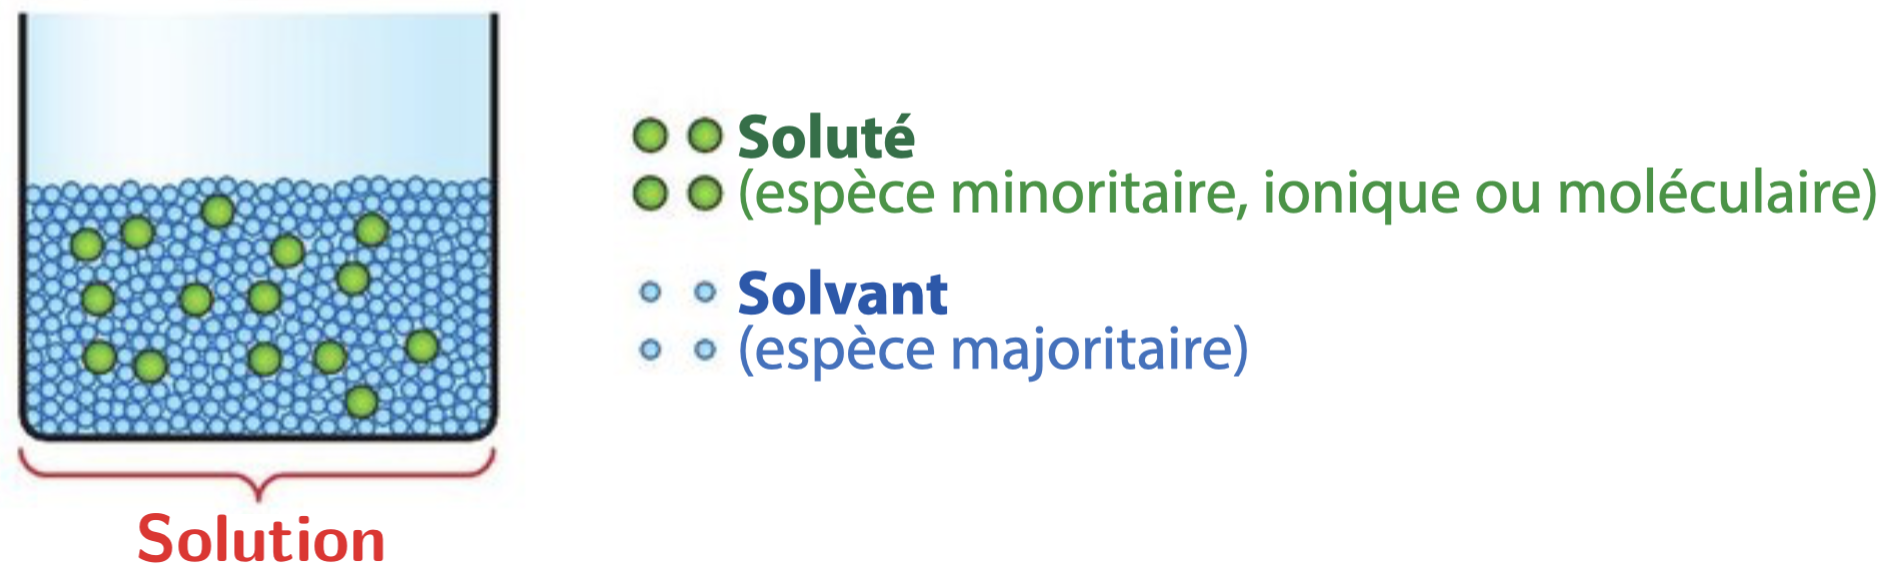
\includegraphics[width=0.5\textwidth]{Images/Solution_solvant.png}
  \end{wrapfigure}
  Une \textbf{solution} est un mélange homogène obtenu par dissolution d’une ou plusieurs espèces chimiques appelées \textbf{solutés} dans une espèce chimique liquide appelé \textbf{solvant}.\\

  Si le solvant est l'eau, on parle de \textbf{solution acqueuse}.
\end{tcolorbox}
\begin{tcolorbox}[colback=green!5!white,colframe=green!75!black,title=\textbf{Concentration en masse}]
La \textbf{concentration en masse}, notée $C_m$,  d’un soluté dans une solution correspond à la masse de soluté dissous dans un litre de solution. Elle s’exprime par exemple en gramme par litre (g.L$^{-1}$).

\end{tcolorbox}

\end{doc}
\newpage
\begin{doc}{Données utiles sur quatre boissons sucrées}
\begin{center}
    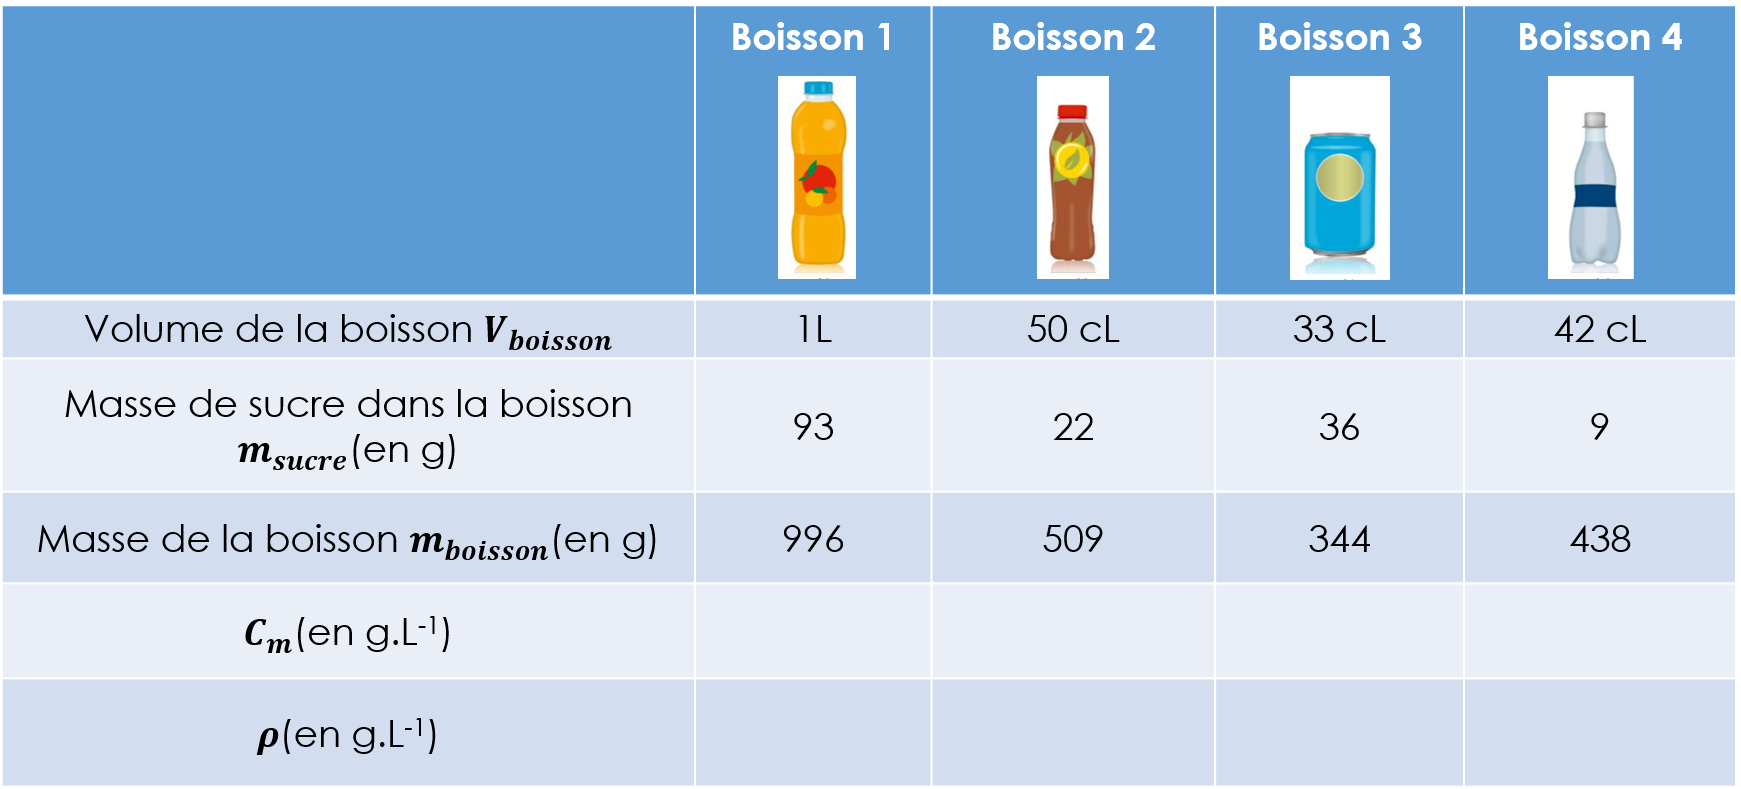
\includegraphics[scale=0.5]{Images/Donnees.png}
\end{center}
\end{doc}

\question{Identifier le solvant et un des solutés des boissons du document 2.}{Le solvant est l'eau, les boissons sont donc des solutions acqueuses. Un soluté de la solution est le sucre car le sucre est minoritaire par rapport à l'eau.}{0}

\question{Calculer la concentration en masse de sucre $C_m$ dans chacune des boissons du document 2 en g.L$^{-1}$. Noter les résultats obtenus dans l’avant-dernière ligne du tableau de ce document.}{\begin{enumerate}
    \item Pour la boisson 1, $C_m=\frac{93}{1}=93$~g.L$^{-1}$,
    \item Pour la boisson 2, $C_m=\frac{22}{0,50}=44$~g.L$^{-1}$,
    \item Pour la boisson 3, $C_m=\frac{36}{0,33}=109$~g.L$^{-1}$,
    \item  Pour la boisson 4, $C_m=\frac{9}{0,42}=21$~g.L$^{-1}$,
\end{enumerate}}{0}

\question{Sachant qu'un morceau de sucre pèse 4,5 grammes, combien de morceaux de sucre contient la boisson la moins sucrée ? La boisson la plus sucrée ?}{La boisson la moins sucrée est la n$^\circ$4. Elle contient $\frac{9}{4,5}=2$ morceaux de sucre. La boisson la plus sucrée est la n$^\circ$3. Elle contient environ $\frac{36}{4,5}=8$ morceaux de sucre.}{0}

\question{Formuler une expression mathématique pour calculer la concentration en masse $C_m$ à partir de la masse de soluté $m_{\text{soluté}}$ et du volume $V_{solution}$ de la solution.}{En raisonnant sur les unités, on a :
\begin{equation*}
    C_m = \frac{m_{\text{soluté}}}{V_{\text{solution}}}
\end{equation*}}{0}

\question{Rappeler l’expression de la masse volumique $\rho$ d’un échantillon en précisant le nom des grandeurs utilisées.}{D'après le cours du Chapitre 1 : \begin{equation*}
    \rho = \frac{m_{boisson}}{V_{boisson}}
\end{equation*}}{0}

\question{Calculer la masse volumique $\rho$ de chacune des boissons du document 2 en g.L$^{-1}$. Noter les résultats obtenus dans la dernière ligne du tableau.}{\begin{enumerate}
    \item Pour la boisson 1, $\rho=\frac{996}{1}=996$~g.L$^{-1}$,
    \item Pour la boisson 2, $\rho=\frac{509}{0,50}=1018$~g.L$^{-1}$,
    \item Pour la boisson 3, $\rho=\frac{334}{0,33}=1012$~g.L$^{-1}$,
    \item  Pour la boisson 4, $\rho=\frac{438}{0,42}=1043$~g.L$^{-1}$.
    \end{enumerate}}{0}

\question{La concentration en masse $C_m$ d’un soluté dans une solution et la masse volumique $\rho$ d’une solution sont deux grandeurs distinctes qui peuvent être données dans la même unité (en g.L$^{-1}$ par exemple). Expliquer la différence entre la concentration en masse et la masse volumique.}{La concentration en masse permet de déterminer la masse d'un soluté contenue dans une solution. La masse volumique d'une solution est une propriété physique de la solution. Elle permet de savoir quelle sera la masse de la solution pour un volume donné}{0}

  %%%%%%%%%% TP %%%%%%%%%%%%%%%
  %%%%% début de la page

\renewcommand{\thesubsection}{\textcolor{red}{\Roman{section}.\arabic{subsection}}}
\renewcommand{\thesubsubsection}{\textcolor{red}{\Roman{section}.\arabic{subsection}.\alph{subsubsection}}}

\setcounter{section}{0}
\setcounter{document}{0}
\sndEnTeteTPQuatre

\begin{center}
\begin{mdframed}[style=titr, leftmargin=60pt, rightmargin=60pt, innertopmargin=7pt, innerbottommargin=7pt, innerrightmargin=8pt, innerleftmargin=8pt]

\begin{center}
\large{\textbf{TP 4 : Comment bien choisir la verrerie pour mesurer des volumes précis ?}}
\end{center}


\end{mdframed}
\end{center}

%\begin{tableauCompetences}
 %   ANA & Mesurer des volumes & & & &
    
%\end{tableauCompetences}

%%%% objectifs
\begin{tcolorbox}[colback=blue!5!white,colframe=blue!75!black,title=Objectifs de la séance :]
\begin{itemize}
    \item Mesurer des masses pour étudier la variabilité du volume mesuré par une pièce de verrerie
  %\item Choisir et utiliser la verrerie adaptée pour préparer une solution par dissolution
\end{itemize}
\end{tcolorbox}

%%%% contexte

\begin{tcolorbox}[colback=orange!5!white,colframe=orange!75!black,title= Scénario:]
Le laboratoire dispose de trois principales pièces de verrerie qu'on utilise couramment lors de manipulation complexe. Nommer ces trois verreries.
\begin{center}
    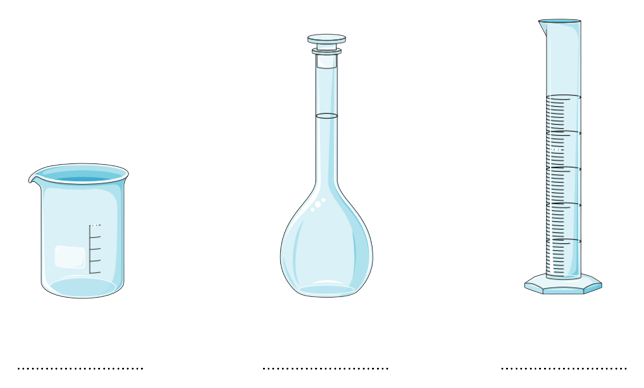
\includegraphics[scale=0.7]{Images/Verrerie_a_completer.png}
\end{center}
\problematique{On souhaite vérifier que la fiole jaugée est la pièce de verrerie la plus précise et la plus fidèle. Comment fait-on ?}
\end{tcolorbox}

\begin{tcolorbox}[colback=red!5!white,colframe=red!75!black,title= Consignes :]
\begin{itemize}
    \item Vous travaillez collaborativement par rangées de 2 binômes,
    \item Dans chaque binôme, nommer un responsable \og MES \fg : il aura la responsabilité de vérifier la bonne réalisation des mesures et de rentrer les valeurs expérimentales sur le fichier Excel du tableau. Nommer également un responsable \og COM \fg : il aura la responsabilité du compte-rendu et fera office de porte-parole du binôme,
    \item Faire attention à la verrerie lors de son utilisation,
    \item Respectez les consignes d'utilisation de la salle de chimie.
\end{itemize}

\end{tcolorbox}
\begin{mdframed}[style=autreexo]
\textbf{\bsc{Liste du matériel}}
\vspace{-0.5cm}
\begin{multicols}{2}
\begin{itemize}
    \item une balance, 
    \item un bécher de 50~mL
    \item un bécher de 100~mL,
    \item une fiole jaugée de 100~mL,
    \item une éprouvette graduée de 100~mL,
    \item une pipette plastique,
    \item une pissette d'eau distillée,
    \item un ordinateur avec le tableur Excel.    
\end{itemize}
\end{multicols}
\end{mdframed}

\newpage
%%%% documents
\begin{doc}{Lecture d'un volume sur la verrerie}

\begin{wrapfigure}{r}{0.3\textwidth}
\vspace{-2cm}
    \centering
      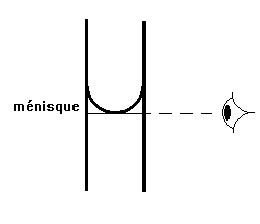
\includegraphics[width=0.27\textwidth]{Images/Lecture_Verrerie.png}
  \end{wrapfigure}
  Lorsqu'on verse un liquide dans une pièce de verrerie (éprouvette, tube à essai, etc), il se forme un ménisque qui va perturber la lecture du volume sur la verrerie. Pour lire le volume occupé par un liquide, il faut positionner son \oe il sur le bas du ménisque.
\end{doc}

%%%%
\begin{doc}{Protocole de remplissage d'une fiole jaugée}
  \label{doc:fiole_jaugee}
  \begin{center}
      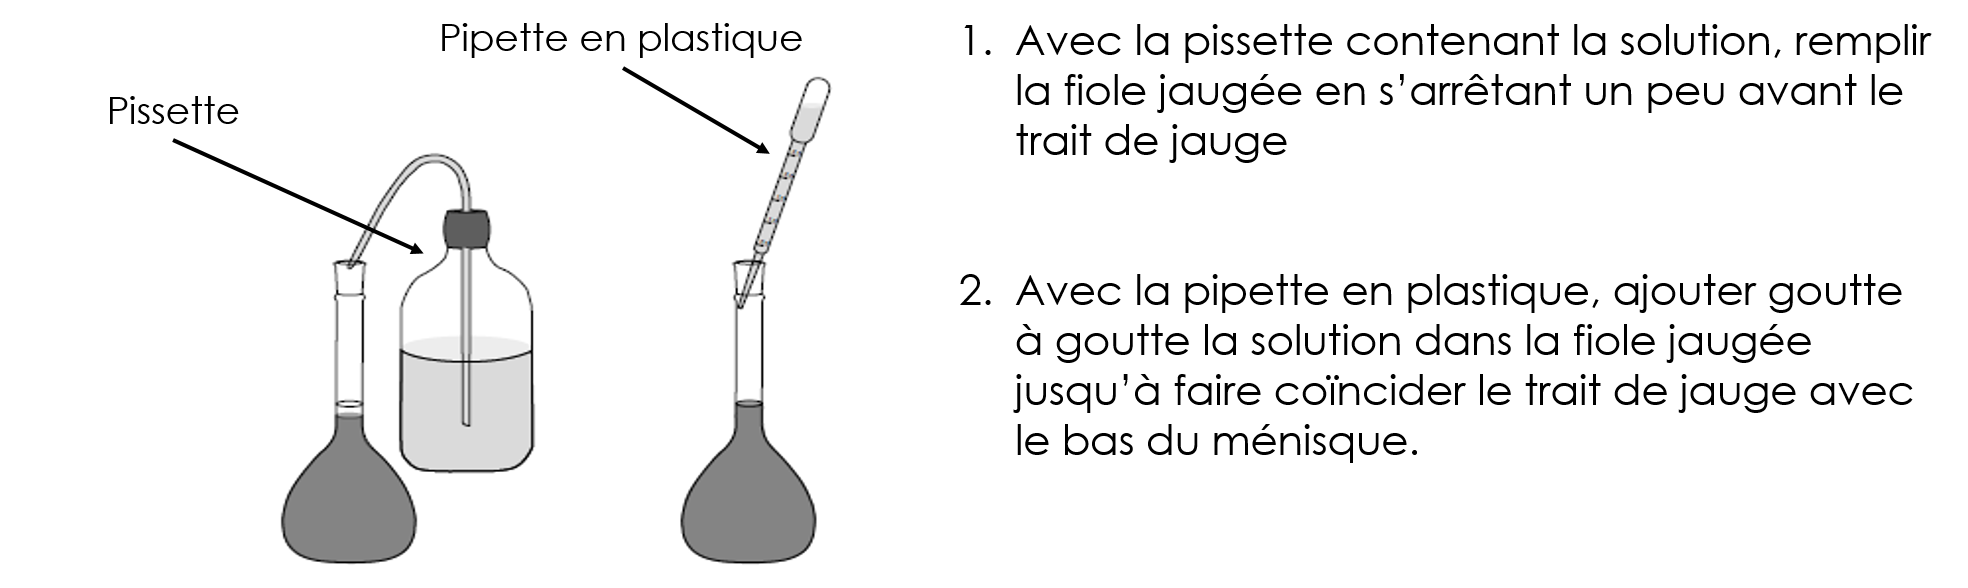
\includegraphics[scale=0.5]{Images/Protocole_fiolejaugee.png}
  \end{center}
\end{doc}

%%%%
\begin{large}
    \textbf{\textcolor{red}{\underline{Travail à réaliser :}}}
\end{large}

\question{Récupérer le fichier \og TP4Resultats.xlsx \fg~dans le dossier de votre classe sur l'ENT dans l'application \og Espace Documentaire \fg. }{~}{0}
\question{Comment réaliser la mesure d'un volume d'eau distillée avec une balance ? Vous écrirez le protocole expérimental sur votre compte-rendu \underline{avec la formule que vous utiliserez}.}{On connaît la masse volumique de l'eau $\rho_{eau}=\frac{m}{V}=1$~g.mL$^{-1}$. En pesant la masse d'eau contenue dans la verrerie (après avoir soustrait la masse de la verrerie bien sûr), on en déduit immédiatemement le volume d'eau}{0}

\question{Pour chaque type de verrerie, réaliser 3 fois la mesure d'un volume de 100~mL d'eau distillée. Compléter le tableau suivant avec vos résultats :
\begin{center}
    \begin{tabular}{|c|C{0.2}|C{0.2}|C{0.2}|}
    \hline
         Verrerie & Mesure n°1 & Mesure n°2 & Mesure n°3  \\
         \hline
         \cellcolor{blue!25} Bécher &   &  & \\
         \hline
         \cellcolor{blue!25} \'{E}prouvette graduée &   &   &\\ 
         \hline
         \cellcolor{blue!25} Fiole jaugée &   &   &\\
         \hline
    \end{tabular}
\end{center}}{Blabla}{0}

\question{Rentrer vos valeurs dans votre tableur Excel et dans celui du binôme de votre rangée.}{~}{0}
\question{Le responsable MES vient compléter avec ses mesures le tableau Excel au tableau.}{~}{0}
\question{Avec les fonctions MOYENNE et ECART-TYPE du tableur Excel, calculer la valeur moyenne et l'écart-type pour chaque verrerie.}{~}{0}
\question{Imprimer les graphiques de vos mesures pour chaque verrerie : sélectionner les 3 graphiques, cliquer sur Fichier-> Imprimer -> Aperçu avant impression.}{~}{0}
\question{Représenter la moyenne et l'écart-type sur vos graphiques.}{~}{0}
\question{A l'aide des moyennes et des écart-types, justifier quelle est la verrerie la plus précise.}{~}{0}
  %\modeCorrection

%%%% début de la page

\renewcommand{\thesubsection}{\textcolor{red}{\Roman{section}.\arabic{subsection}}}
\renewcommand{\thesubsubsection}{\textcolor{red}{\Roman{section}.\arabic{subsection}.\alph{subsubsection}}}

\setcounter{section}{0}
\setcounter{document}{0}
\sndEnTeteTPCinq

\begin{center}
\begin{mdframed}[style=titr, leftmargin=60pt, rightmargin=60pt, innertopmargin=7pt, innerbottommargin=7pt, innerrightmargin=8pt, innerleftmargin=8pt]

\begin{center}
\large{\textbf{TP 5 : Estimation de la concentration d'une solution colorée à l'aide d'une échelle de teintes
}}
\end{center}


\end{mdframed}
\end{center}

%%%% objectifs
\begin{tcolorbox}[colback=blue!5!white,colframe=blue!75!black,title=Objectifs de la séance :]
\begin{itemize}
    \item Réaliser une échelle de teintes
    \item Choisir et utiliser la verrerie adaptée pour préparer une solution par dilution,
    \item Encadrer la valeur d’une concentration en masse à l’aide d’une échelle de teinte.
\end{itemize}
\end{tcolorbox}

%%%% Consignes
\begin{tcolorbox}[colback=red!5!white,colframe=red!75!black,title= Consignes :]
\begin{itemize}
    \item Réaliser le travail en binôme,
    \item Faire attention à la verrerie lors de son utilisation,
    \item Respectez les consignes d'utilisation de la salle de chimie.
\end{itemize}
\end{tcolorbox}

%%%% contexte

\begin{tcolorbox}[colback=orange!5!white,colframe=orange!75!black,title= Scénario:]
\begin{wrapfigure}{r}{0.5\textwidth}
\vspace{-0.6cm}
    \centering
      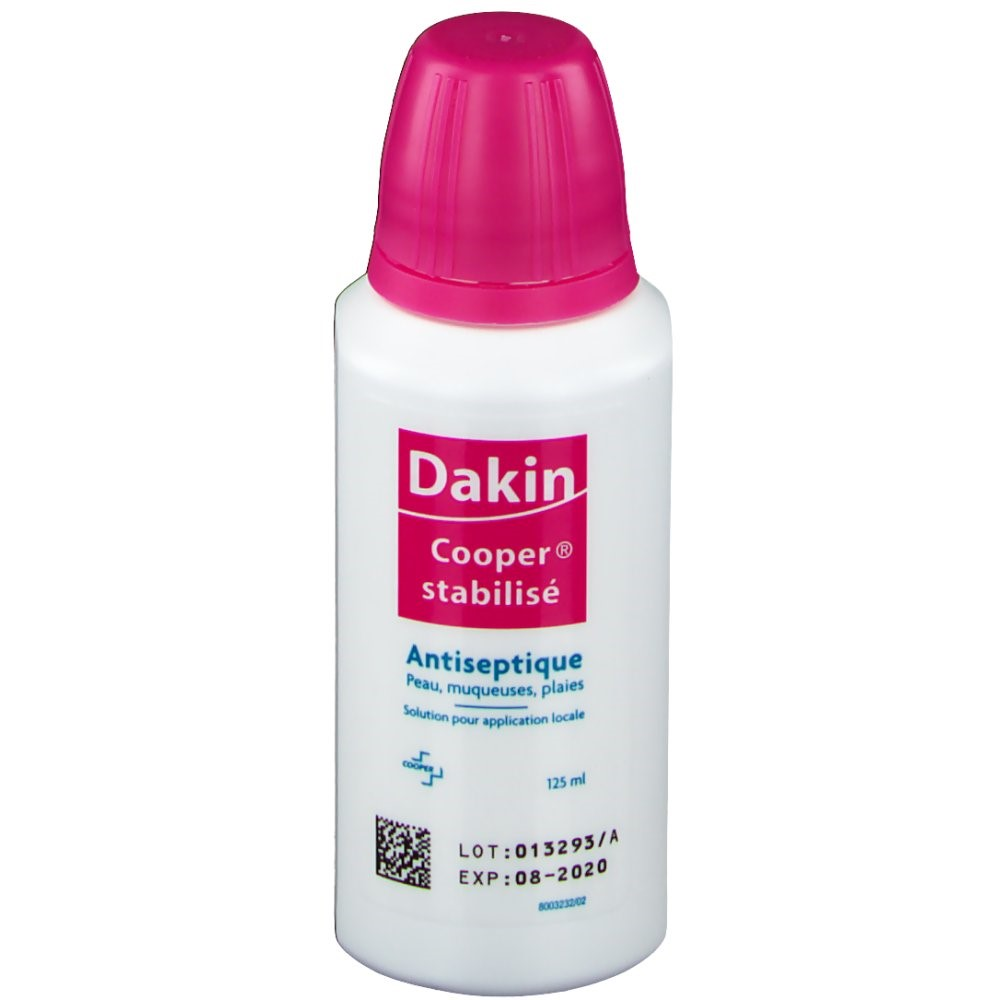
\includegraphics[width=0.4\textwidth]{Images/Dakin.jpg}
  \end{wrapfigure}
L’eau de Dakin est une solution aqueuse de couleur rose pâle et à l’odeur d’eau de Javel, elle est utilisée pour le lavage de la peau et des muqueuses.\\
C’est au cours de la première guerre mondiale que le chimiste américain Henri Dakin et le chirurgien français Alexis Carrel mettent au point cet antiseptique.\\
L’eau de Dakin est à base d’hypochlorite de sodium \chemform{NaClO}, qui en est le principe actif, et de permanganate de potassium \chemform{KMnO_4}, qui lui donne sa coloration rose et qui permet de stabiliser la solution vis-à-vis de la lumière.\\

\problematique{Afin de s'assurer de la qualité de ce flacon, on souhaite estimer la concentration en masse de permanganate de potassium dans un flacon d’eau de Dakin. Comment fait-on ?}
\end{tcolorbox}
\newpage

\begin{mdframed}[style=autreexo]
\textbf{\bsc{Liste du matériel}}
\begin{itemize}
    \item une solution aqueuse $S_0$ de permanganate de potassium \chemform{KMnO_4} de concentration en masse $C_{m,0}=80$~mg.L$^{-1}$, 
    \item une pissette d'eau distillée,
    \item des béchers,
    \item des pipettes jaaugées de 1mL, 2mL, 5mL, 10mL et 20mL,
    \item des fioles jaugées de 50mL,
    \item des pipettes Pasteur en plastique,
    \item des tubes à essais et leur support.    
\end{itemize}
\end{mdframed}


%%%% documents
\begin{doc}{La dilution}
Le principe est de prélever un certain volume d'une solution concentrée initiale appelée \textcolor{red}{solution mère} puis d'y ajouter de l'eau pour obtenir une solution moins concentrée appelée \textcolor{red}{solution fille} :
\begin{center}
    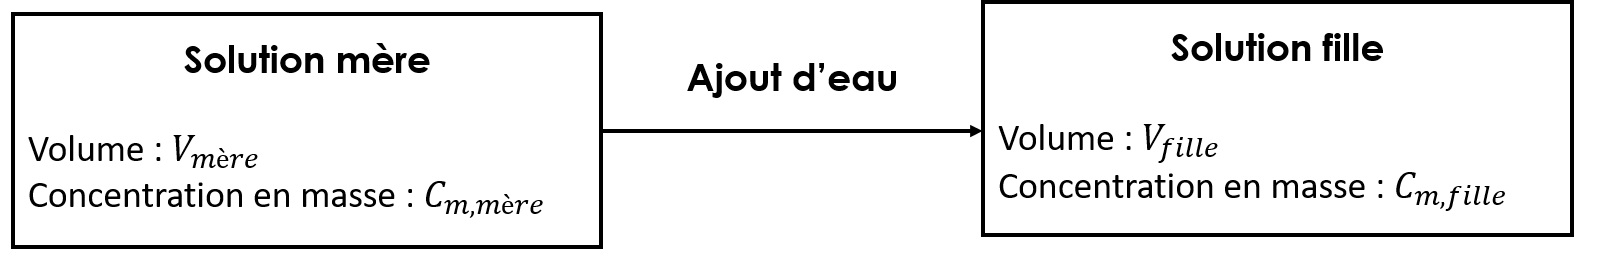
\includegraphics[scale=0.59]{Images/Dilution2.png}
\end{center}
\begin{tcolorbox}[colback=red!5!white,colframe=red!75!black,title=\textbf{Propriété de la dilution : }]
Au cours d'une dilution, la masse de soluté prélevée se conserve :
\begin{empheq}[box=\fbox]{align*}
    m_{\text{prélevée, mère}} &= m_{\text{soluté, fille}}\\
    C_{m,\text{mère}}V_{\text{prélevé}} &= C_{m,fille}V_{\text{fille}}
\end{empheq}
On peut dès lors définir le \textcolor{red}{facteur de dilution}, noté $F$ de la manière suivante :
\begin{equation*}
    F=\frac{C_{m,\text{mère}}}{C_{m,fille}} = \frac{V_{\text{fille}}}{V_{\text{prélevé}}}
\end{equation*}
\end{tcolorbox}
\end{doc}
\newpage
%%%%
\begin{doc}{Protocole expérimental de préparation d'une solution aqueuse par dilution}
\vspace{-0.8cm}
\begin{center}
    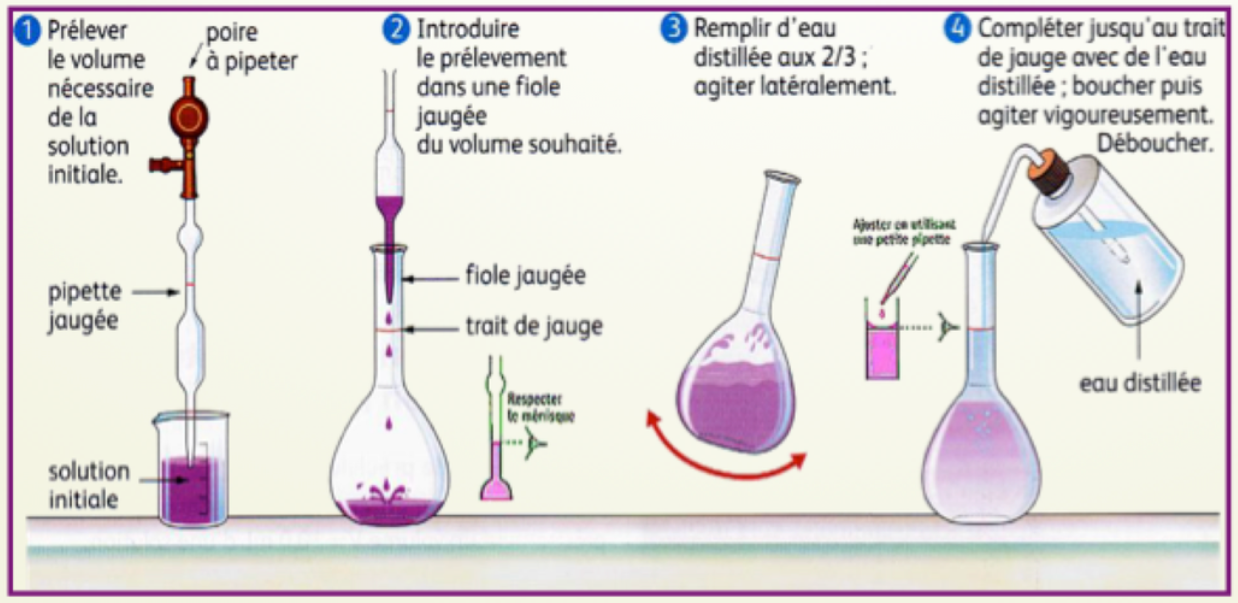
\includegraphics[scale=0.5]{Images/Protocole_dilution.png}
  \end{center}
  
  \begin{enumerate}
    \item Prélever un volume $V_\text{mère}$ de la solution mère à l'aide de la pipette jaugée.
    Le bas du ménisque doit atteindre la graduation supérieure.
    \item Introduire la solution prélevée dans la fiole jaugée de volume $V_\text{fille}$.
    \item Ajouter de l'eau distillée dans la fiole jaugée jusqu'aux $2/3$ et agiter doucement. 
    \item Ajouter goutte à goutte de l'eau distillée avec une pipette Pasteur jusqu'à ce que le bas du ménisque atteigne le trait de jauge (\textcolor{red}{vérifier à l'\oe il}),
    \item Fermer la fiole avec un bouchon et l'agiter en la retournant plusieurs fois.
    \item Verser la solution fille obtenue dans un bécher.
    \end{enumerate}
\end{doc}


%%%%
\newpage
\begin{doc}{\'{E}tiquette d'un flacon d'eau de Dakin commercial}
\vspace{-0.4cm}
  \label{doc:dakin}
  \begin{center}
      \begin{tabular}{|C{0.2}|C{0.25}|C{0.25}|c|}
      \hline
       & Soluté & Concentration en masse & Couleur\\
       \hline 
          Principe actif & Hypochlorite de sodium \chemform{NaClO} & 0,500~g de chlore actif pour 100~mL & Incolore (en solution)\\
          \hline
          \multirow{3}{*}{Principe non actifs} & Permanganate de potassium \chemform{KMnO_4} & 0,0010~g pour 100mL & Violet (en solution)\\
           & Dihydrogénophosphate de sodium déshydraté & Non connue (excipient) & Blanc (solide) \\
           & Eau purifiée & Non connue (excipient) & Incolore\\
           \hline
      \end{tabular}
  \end{center}
\end{doc}
 
%%%%

\begin{large}
    \textbf{\textcolor{red}{\underline{Travail à réaliser :}}}
\end{large}
\\
\question{Identifier le solvant de l'eau de Dakin et un soluté.}{L'eau de Dakin est une solution aqueuse. Par définition, l'eau est le solvant de cette solution.}{0}
\question{Parmis les solutés de l'eau de Dakin, identifier son principe actif et l'espèce chimique responsable de sa couleur.}{D'après le document 3, le principe actif est l'ion hypochlorite de sodium \chemform{NaClO} et l'espèce responsable de la couleur est le permanganate de potassium \chemform{KMnO_4}}{0}
\\
\question{Compléter le document 1 sur la propriété de la dilution.}{Voir le document 1.}{0}
\\
\question{On souhaite préparer quatre solutions, notées S$_{1}$, S$_{2}$, S$_{3}$ et S$_{4}$ à partir de la solution aqueuse S$_{0}$ de permanganate de potassium de concentration en masse $C_{m,0}=80$~mg.L$^{-1}$. Compléter le tableau ci-dessous \textbf{\underline{après avoir détaillé le calcul pour la solution S$_{1}$}} :
\begin{center}
    \begin{tabular}{|c|c|c|c|c|}
        \hline
        Solution fille & V$_{\text{mère à prélever}}$ (en mL) & V$_{\text{fille}}$ (en mL) & $C_{m,fille}$ (en mg.L$^{-1}$) & Facteur de dilution $F$\\
        \hline
         S$_{1}$ & 1  & 50,0  & 1,6 & 50 \\
         \hline
         S$_{2}$ & 2 & 50,0  & 3,2 & 25 \\
         \hline
         S$_{3}$ & 5 & 50,0  & 8,0 & 10 \\
         \hline
         S$_{4}$ & 10  & 50,0  & 16 & 5 \\
         \hline
         \textit{(Bonus)} S$_{5}$ & 15 & 50,0 & 24 & environ 3 \\
         \hline
         \textit{(Bonus)} S$_{6}$ & 20 & 50,0 & 32 & 2,5\\
         \hline
    \end{tabular}
\end{center}
}{}{0}\\
\question{En suivant le protocole du document 2 (et les explications du professeur), préparer les solutions S$_{1}$, S$_{2}$, S$_{3}$ et S$_{4}$.}{Fait en TP.}{0}
\\
\question{\`{A} votre avis, comment feriez-vous pour déterminer la concentration de la solution mère commerciale ?}{Il y a deux possibilités : 
\begin{itemize}
    \item Comme on sait que la solution est colorée et que la couleur provient des ions permanganates, on peut réaliser une échelle de teinte avec différentes concentrations en masse $C_m$ d'ions permanganates et comparer la teinte à celle de la solution commerciale (c'est ce qu'on va faire ici),
    \item mesurer la masse volumique de chaque solution fille et réaliser une courbe d'étalonnage (c'est ce qu'on fera au TP 6).
\end{itemize}}{0}

\question{Remplir sur quelques centimètres les tubes à essais avec vos solutions filles. Attention à se rappeler la correspondance entre la solution dans le tube à essai et la solution $S$ correspondante.}{Effectué en TP.}{0}
\\
\question{Puis, déterminer \textbf{\underline{un encadrement}} de la concentration en masse en permanganate de potassium de la solution d'eau de Dakin commerciale.}{On trouve à l'aide de l'échelle de teintes réalisées : $8~\text{mg.L}^{-1}<C_{m,Dakin} < 16~\text{mg.L}^{-1}$}{0}
\\
\question{\`{A} partir des données de l'étiquette de la solution commerciale, calculer la concentration en masse de permanganate de potassium normalement présente dans la solution commerciale.}{Les données de l'étiquette donnent une concentration en masse égale à $C_{m,Dakin}=\frac{0,0010~\text{g}}{100~\text{mL}}=\frac{1,0~\text{mg}}{0,1~\text{L}}=10~\text{mg.L}^{-1}$}{0}
\\
\question{Vos résultats expérimentaux sont-ils en accord avec cette concentration en masse ? }{Oui, l'encadrement donne une concentration en masse de permanganate dans la solution de Dakin entre 8 et 16~mg.L$^{-1}$. Cet encadrement contient bien la valeur de $C_{m,Dakin}=10~\text{mg.L}^{-1}$.}{0}

\begin{center}
    \includegraphics[scale=0.9]{Images/Grands_carreaux.pdf}
\end{center}

  %\modeCorrection

%%%% début de la page

\renewcommand{\thesubsection}{\textcolor{red}{\Roman{section}.\arabic{subsection}}}
\renewcommand{\thesubsubsection}{\textcolor{red}{\Roman{section}.\arabic{subsection}.\alph{subsubsection}}}

\setcounter{section}{0}
\setcounter{document}{0}
\sndEnTeteTPSix

\begin{center}
\begin{mdframed}[style=titr, leftmargin=60pt, rightmargin=60pt, innertopmargin=7pt, innerbottommargin=7pt, innerrightmargin=8pt, innerleftmargin=8pt]

\begin{center}
\large{\textbf{TP 6 : Les sodas sont-ils trop sucrés ?
}}
\end{center}
\end{mdframed}
\end{center}

\begin{tableauCompetences}
    APP & Exploiter des explications orales pour rédiger un protocole & & & & \\
    \hline
    REA & Réaliser une série de mesures ; relever les résultats obtenus & & & & \\
     \hline 
     REA & Utiliser une grandeur quotient pour déterminer le numérateur ou le dénominateur& & & & \\
     \hline 
    COM & Rendre compte de façon écrite & & & & \\
    \hline
    VAL & Analyser l’ensemble des résultats de façon critique  & & & &
\end{tableauCompetences}


%%%% objectifs
\begin{tcolorbox}[colback=blue!5!white,colframe=blue!75!black,title=Objectifs de la séance :]
\begin{itemize}
    \item Choisir et utiliser la verrerie adaptée pour préparer une solution par dissolution,
    \item Réaliser une courbe d'étalonnage,
    \item Déterminer la valeur d’une concentration en masse à partir de résultats expérimentaux.
\end{itemize}
\end{tcolorbox}

%%%% Consignes
\begin{tcolorbox}[colback=red!5!white,colframe=red!75!black,title= Consignes :]
\begin{itemize}
    \item Rendre un compte-rendu par binôme en fin de TP,
    \item Faire attention à la verrerie lors de son utilisation,
    \item Respectez les consignes d'utilisation de la salle de chimie.
\end{itemize}
\end{tcolorbox}

%%%% contexte

\begin{tcolorbox}[colback=orange!5!white,colframe=orange!75!black,title= Scénario:]
\begin{wrapfigure}{r}{0.4\textwidth}
\vspace{-0.6cm}
    \centering
      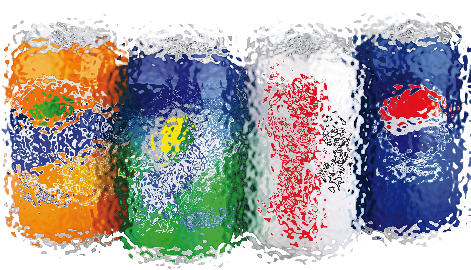
\includegraphics[width=0.4\textwidth]{Images/Soda_flou.png}
  \end{wrapfigure}
La consommation de soda dans le monde est gigantesque. Pour la marque Coca-cola, des études statistiques estiment que la consommation moyenne de ce soda est d'environ 350 milliards de litres par jour.\\
Les sodas sont des boissons gazeuses pour la plupart très sucrées pouvant causer une maladie qu'on a pu nommer que très récemment : la maladie du soda ou maladie du foie gras. Cette maladie cause des effets très sévères à moyen et long terme : diabète de type 2, excès de graisse dans le foie, ... Une étude pilotée par l'INSERM (Institut National de la Santé et de la Recherche Médicale) a montré que près d’un français sur cinq (18,2\%) présente un excès de graisse dans le foie.

\problematique{Quelle est la concentration en masse de sucre dans une bouteille de soda de marque bien connue ?}
\end{tcolorbox}
\newpage

\begin{mdframed}[style=autreexo]
\textbf{\bsc{Liste du matériel}}
\begin{itemize}
    \item Spatule ;
    \item Balance ;
    \item Fiole jaugée de 100,0 mL ;
    \item Béchers ;
    \item Entonnoir en plastique ;
    \item Une bouteille de soda dégazée ;
    \item Sucre ;
    \item Eau ;
    \item Logiciel tableur-grapheur (Excel) ; 
\end{itemize}
\end{mdframed}

\begin{doc}{\'{E}tiquette d'une bouteille de soda d'une marque bien connue}
\vspace{-0.4cm}
  \label{doc:Coca}
  \begin{center}
     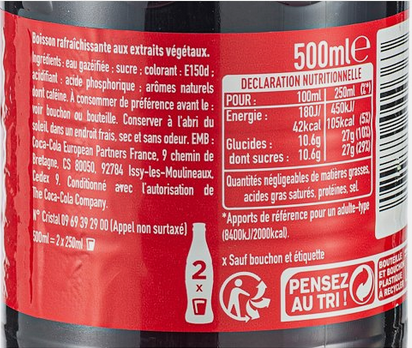
\includegraphics[scale=2]{Images/Etiquette_coca.png}
  \end{center}
\end{doc}
 
%%%%
\newpage

%%%% documents
\begin{doc}{Utilisation d'une courbe d'étalonnage}
Une courbe d'étalonnage permet de relier deux grandeurs mesurables (par exemple la masse volumique et la concentration en masse). \\
L'idée est de fabriquer des \textcolor{red}{solutions étalons} avec des propriétés (masse volumique, concentration en masse, ...) que l'expérimentateur choisit puis mesure : ce sont les croix noires sur le graphique ci-dessous. Ensuite, on mesure une grandeur d'une solution inconnue (par exemple sa masse volumique) qu'on place sur la courbe d'étalonnage pour en déduire l'autre grandeur (par exemple sa concentration en masse) : c'est la croix bleue sur le graphique ci-dessous.
\begin{center}
    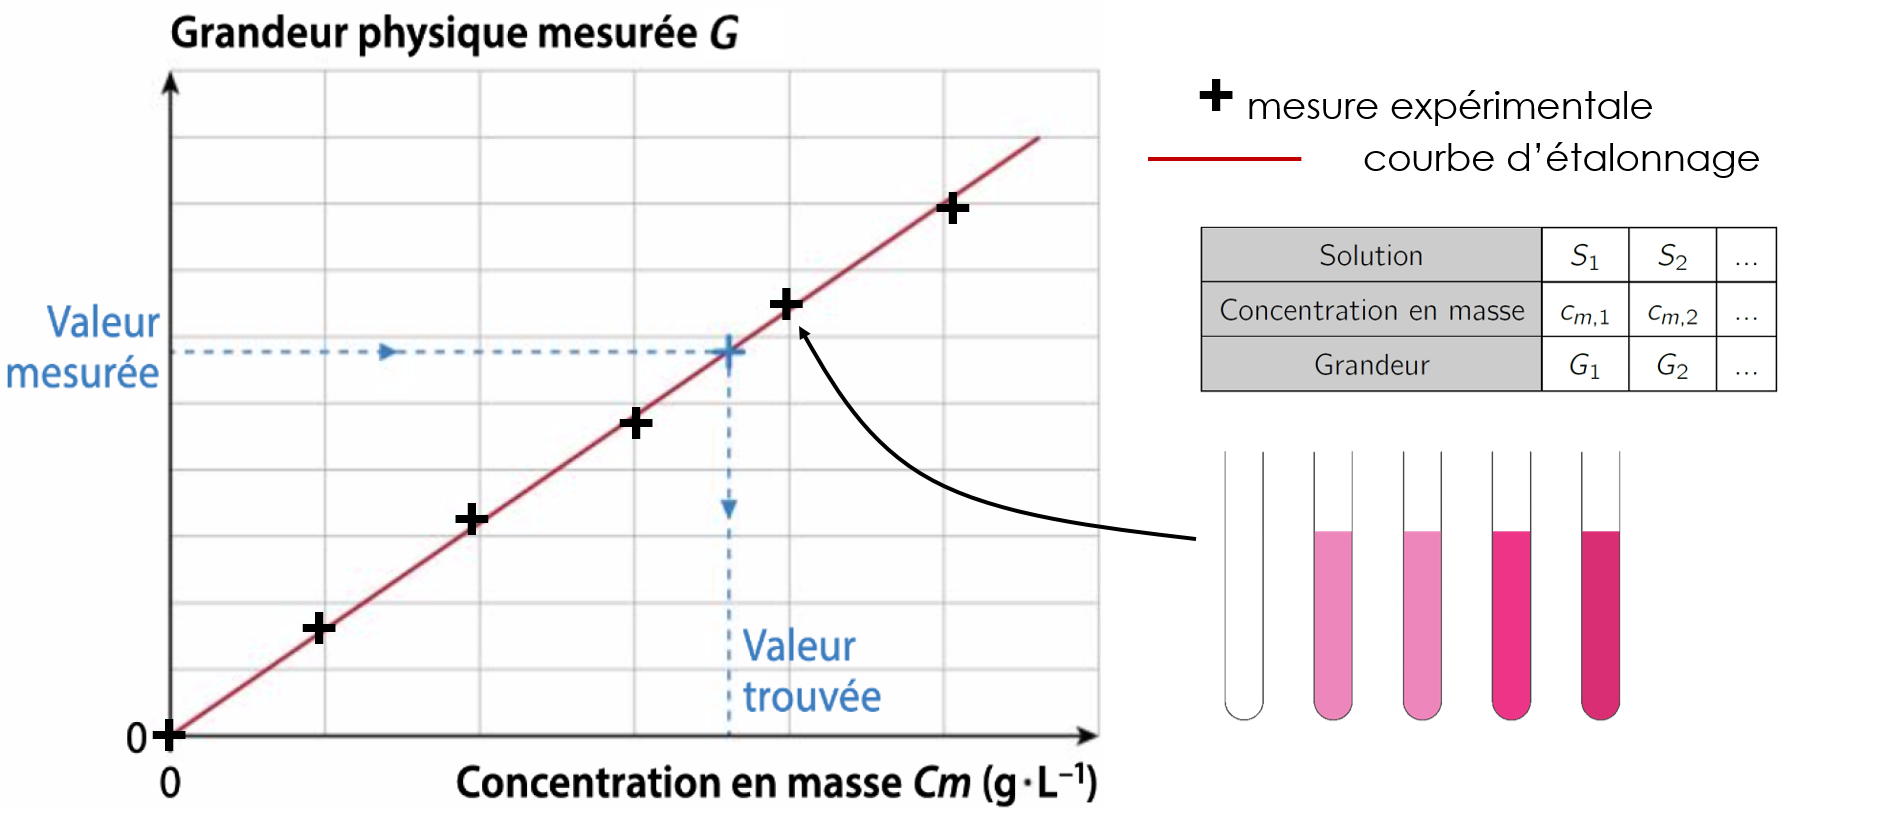
\includegraphics[scale=0.5]{Images/Courbe_etalonnage.png}
\end{center}
On peut connaître la valeur recherchée soit par une lecture graphique, soit à l'aide d'une \textcolor{red}{courbe d'étalonnage} (courbe rouge sur le graphique ci-dessus) qui représente une modélisation mathématique du lien entre les deux grandeurs mesurées (une relation linéaire sur le grahique ci-dessus).
\end{doc}
%%%%
\begin{doc}{Protocole expérimental de préparation d'une solution aqueuse par dissolution}
\vspace{-0.8cm}
\begin{center}
    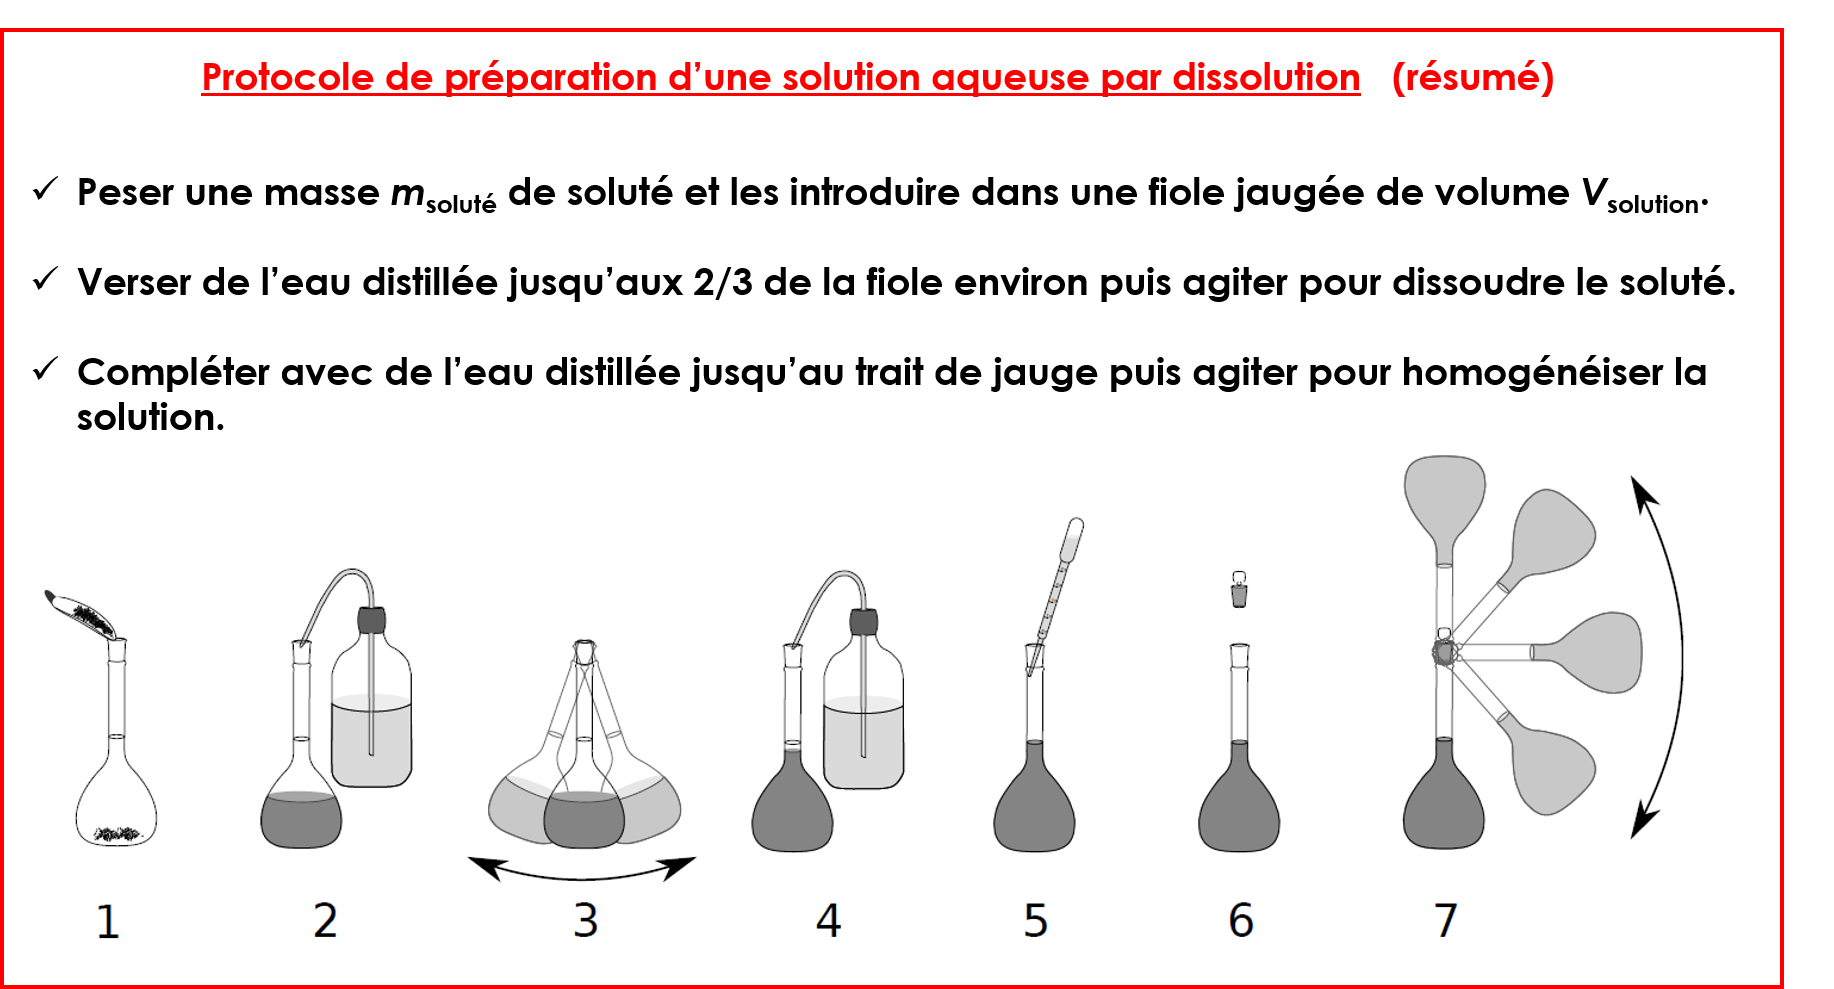
\includegraphics[scale=0.5]{Images/Dissolution.png}
  \end{center}

\end{doc}

%%%%
\newpage
%%%%
\begin{large}
    \textbf{\textcolor{red}{\underline{Travail à réaliser :}}}
\end{large}
\\
\question{Télécharger le fichier \og \text{TP6\_Coca\_Resultats.xlsx}~\fg ~depuis l'ENT dans l'application "Espace Documentaire". Vous l'enregistrerez sur le bureau de votre session.}{~}{0}
\\
\question{Déterminer le solvant et au moins deux solutés dans le soda de marque bien connue.}{D'après le document \ref{doc:Coca}, le solvant est l'eau et deux solutés possibles sont : le sucre et le colorant E150d.}{0}
\\
\question{Déterminer la concentration en masse de sucre dans le soda à l'aide de l'étiquette de la bouteille de soda. On donnera le résultat en g.L$^{-1}$.}{On lit qu'il y a $m=10,6$~g de sucre pour $V=100$~mL de boisson soit une concentration en masse de sucre égale à $C_m= \frac{m}{V}=\frac{10,6}{0,100}=106$~g.L$^{-1}$.}{0}
\\
\question{\'{A} l'aide des explications et de l'expérience réalisée par le professeur, écrire votre protocole expérimental pour réaliser la dissolution d'une masse $m_{sucre}$ de sucre dans un volume $V$. \textbf{\underline{Attention de bien nommer la verrerie}} utilisée à chaque étape du protocole.}{Voici les étapes pour réaliser le protocole de dissolution :
\begin{enumerate}
    \item Peser la fiole jaugée, noter sa masse ;
    \item Mettre un entonnoir en plastique sur la fiole. Placer le tout sur la balance puis tarer la balance ;
    \item \`{A} l'aide d'une spatule, verser une masse $m_{sucre}$ de sucre dans l'entonnoir. Noter la valeur $m_{sucre}$ ;
    \item Rincer l'entonnoir à l'aide d'une pissette d'eau distillée ;
    \item Retirer l'entonnoir puis compléter jusqu'au 2/3 la fiole jaugée d'eau distillée ;
    \item Agiter la fiole pour dissoudre le sucre ;
    \item Compléter la fiole jaugée jusqu'au trait de jauge à l'aide d'une pipette pasteur ;
    \item Placer un bouchon et retourner plusieurs fois la fiole jaugée pour homogénéiser le mélange ;
    \item Peser la masse de l'ensemble \{fiole sans bouchon + solution d'eau sucrée\} et retirer la masse de la fiole jaugée pour en déduire la masse de solution d'eau sucrée ;
\end{enumerate}}{0}
%
\question{Calculer la masse de sucre à peser pour réaliser une solution d'eau sucrée de concentration en masse de sucre $C_{1}=55$~g.L$^{-1}$ de volume $V=100,0$~mL. \textbf{\underline{Expliciter clairement le détail du calcul.}}}{On cherche la masse $m_{sucre}$ telle que $C_m=55$~g.L$^{-1}$. D'après le cours et en utilisant les notations de la question, on sait que :
\begin{equation*}
    C_m = \frac{m_{sucre}}{V}
\end{equation*}
On en déduit donc :
\begin{equation*}
    m_{sucre} = C_m \times V = 55\times 0,100 = 5,5~\text{g}
\end{equation*}
On doit donc peser 5,5~g de sucre pour obtenir une telle solution.}{0}
\\
\question{Sans détailler les calculs, compléter le tableau suivant pour la masse de sucre :
\begin{center}
    \begin{tabular}{|c|C{0.15}|C{0.3}|C{0.1}|C{0.2}|}
    \hline
         Solution & Masse de sucre (en g) & Concentration en masse de sucre $C_m$ (en g.L$^{-1}$) & Volume (en mL) & Masse volumique $\rho$ (en g.L$^{-1}$) \\
         \hline
         $S_1$ & & 55 & 100,0 &\\
         \hline
         $S_2$ & & 75 & 100,0 & \\
         \hline
         $S_3$ & & 95 & 100,0 & \\
         \hline 
         $S_4$ & & 120 & 100,0 & \\
         \hline
    \end{tabular}
\end{center}}{\begin{center}
    \begin{tabular}{|c|C{0.15}|C{0.3}|C{0.1}|C{0.2}|}
    \hline
         Solution & Masse de sucre (en g) & Concentration en masse de sucre $C_m$ (en g.L$^{-1}$) & Volume (en mL) & Masse volumique $\rho$ (en g.L$^{-1}$)\\
         \hline
         $S_1$ & 5,5 & 55 & 100,0 & 1022 \\
         \hline
         $S_2$ & 7,5 & 75 & 100,0 & 1029 \\
         \hline
         $S_3$ & 9,5 & 95 & 100,0 & 1037 \\
         \hline 
         $S_4$ & 11,5 & 120 & 100,0 & 1046 \\
         \hline
    \end{tabular}
\end{center}}{0}

\question{Réaliser les solutions $S_1$ et $S_2$ pour les groupes A et les solutions $S_3$ et $S_4$ pour les groupes B.}{Travail en classe}{0}
\\
\question{Mesurer les masses volumiques de vos solutions et compléter le tableau de la question 6.}{Voir la question 4.}{0}
\\
\question{Reporter vos valeurs dans le tableur Excel. Tracer la courbe (ici une droite) d'étalonnage puis imprimer votre graphique que vous collerez dans votre compte-rendu.}{\begin{center}
    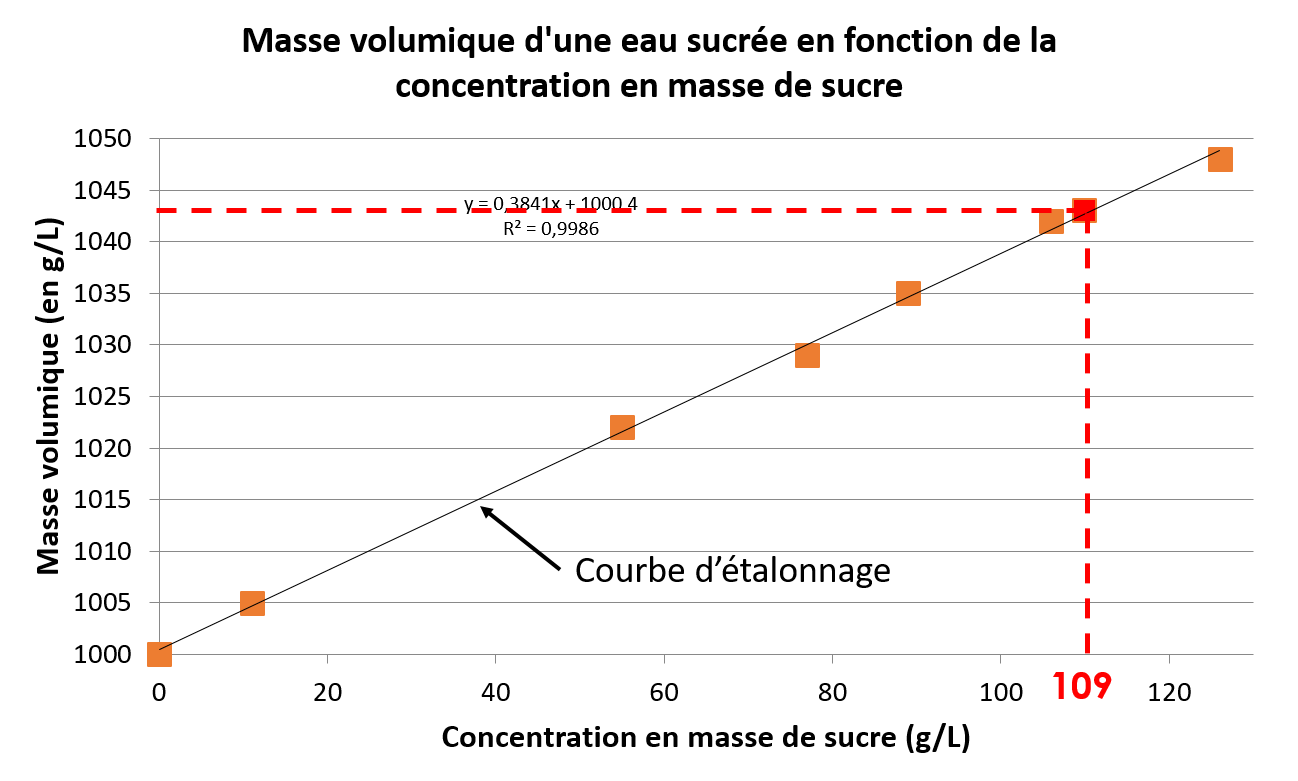
\includegraphics[scale=0.5]{Images/Resultat_coca.png}
\end{center}}{0}
\question{Mesurer la masse volumique du soda, notée $\rho_{soda}$. Placer ce point sur votre courbe d'étalonnage.}{On verse 100,0~mL de soda dans une fiole jaugée dont on connaît la masse. On mesure la masse du liquide introduit et on détermine sa masse volumique. On trouve $\rho_{soda}=1043$~g.L$^{-1}$ qu'on place sur le graphique (carré rouge sur le graphique de la question 8).}{0}
\\
\question{En déduire la concentration en masse $C_{m}^{soda}$ de sucre dans le soda de marque bien connue.}{On en déduit par lecture graphique $C_{m}^{soda}=109$~g.L$^{-1}$.}{0}
\\
\question{Comparer la concentration en masse de sucre obtenue de vos mesures à celle donnée sur l'étiquette de la bouteille de soda. Proposer une explication sur la différence/la similitude entre votre résultat et celui attendu.}{On trouve une valeur très proche de celle donnée sur l'étiquette. Néanmoins nos mesures permettent de montrer que le résultat est légèrement différent (écart de 2,3\%). C'est normal puisque dans le soda, il y a d'autres ingrédients que le sucre (dont les concentrations en masse nous sont inconnues, secret d'entreprise !).}{0}
\\
\question{\textit{(Bonus)} L'OMS (Organisation Mondiale de la Santé) recommande de ne pas consommer plus de 100~g de sucre par jour pour rester en bonne santé, calculer combien de verres de $V=12,5$~cL du soda étudié un être humain peut consommer par jour.}{Un verre de 12,5~cL possède $m=C_m^{soda}\times V = 106\times 0,125=12,7$~g. Un être humain peut donc consommer environ $\frac{100}{12,7}\sim8$ verres de soda par jour \textbf{\underline{si son apport en sucre dans la journée provient}} \textbf{\underline{uniquement du soda}}.}{0}
\\
\question{\textit{(Bonus)} Quelle serait la valeur de la masse volumique d'une solution si la concentration en masse de sucre était égale à $C_{m}=0$~g.L$^{-1}$ ? Vous donnerez le résultat en g.L$^{-1}$.}{On aurait une solution composée d'un volume de 100,0~mL d'eau distillée, sa masse volumique serait donc celle de l'eau soit $\rho_{eau}=1000$~g.L$^{-1}$.}{0}
%\begin{center}
%    \includegraphics[scale=0.75]{Images/Feuilles/Grands_carreaux.pdf}
%\end{center}

%\begin{center}
 %   \includegraphics[scale=0.85]{Images/Feuilles/Grands_carreaux.pdf}
%\end{center}

  %%%%%%%%%% Devoirs Notés %%%%%%%%%%
  \modeCorrection


\renewcommand{\thesubsection}{\textcolor{red}{\Roman{section}.\arabic{subsection}}}
\renewcommand{\thesubsubsection}{\textcolor{red}{\Roman{section}.\arabic{subsection}.\alph{subsubsection}}}
\renewcommand{\titreDocu}[1]{
  \refstepcounter{document} % update counter
  \textbf{Exercice \arabic{document} -- #1} 
  \addcontentsline{toc}{document}{\protect\numberline{} #1} % update table of content
}

\setcounter{section}{0}
\setcounter{document}{0}


\nomPrenomClasse
\vspace{1cm}

\begin{center}
\begin{mdframed}[style=titr, leftmargin=60pt, rightmargin=60pt, innertopmargin=7pt, innerbottommargin=7pt, innerrightmargin=8pt, innerleftmargin=8pt]
\begin{center}
\begin{Large}
    Devoir Surveillé n°2 : Solutions aqueuses (30min)
\end{Large}
\end{center}
\end{mdframed}
\end{center}
\vspace{1cm}

\begin{tableauCompetences}
    APP & S'approprier les informations d'un document & & & & \\
    \hline
    REA & Utiliser une grandeur quotient 
pour déterminer le numérateur ou le dénominateur  & & & & \\
\hline
    ANA &  Exploiter les informations extraites des données & & & & 
\end{tableauCompetences}

\begin{tcolorbox}[colback=red!5!white,colframe=red!75!black,title=\textbf{Consignes : }]
   \begin{enumerate}
        \item Vous rédigez tout sur le sujet,
        \item N'oubliez pas les unités dans vos résultats, 
        \item La calculatrice \underline{n'est pas autorisée}.
   \end{enumerate}
\end{tcolorbox}

\begin{doc}{Quizz \begin{large}
    /6,5 points
\end{large}}
Entourer \underline{la ou les} bonne(s) réponse(s) :
\begin{enumerate}
    \item \textbf{Le sang est un liquide dont l'eau est : (1pt)}
        \begin{align*}
            %a.& ~\text{le soluté} & b.& ~\text{ le solvant} & c.& ~\text{la solution}
            a.& ~\text{le soluté} & b.& ~\text{ \textcolor{red}{le solvant}} & c.& ~\text{la solution}
        \end{align*}
    \item \textbf{Un échantillon de 10 g d’aspirine est dissous dans 50 cL d’eau. La concentration
en masse d’aspirine dans la solution acqueuse est : (1pt)}
        \begin{align*}
            %a.& \text{ 20 g.L$^{-1}$} & b.& \text{ 0,2 g.L$^{-1}$} & c.& ~\text{ 200 g.L$^{-1}$}
            a.& \text{ \textcolor{red}{20 g.L$^{-1}$}} & b.& \text{ 0,2 g.L$^{-1}$} & c.& ~\text{ 200 g.L$^{-1}$}
        \end{align*}
    \item \textbf{On place un cachet de 1000 mg d'aspirine dans un verre contenant un volume de 25 cL d'eau. On agite avec une cuillère. On a réalisé : (1,5pts) }
        \begin{align*}
            %a.& ~\text{Une dilution} & b.& ~\text{Une dissolution} & c.& ~\text{Une solution fille} & d.& ~\text{Une solution aqueuse}
            a.& ~\text{Une dilution} & b.& ~\text{\textcolor{red}{Une dissolution (1pt)} } & c.& ~\text{Une solution fille} & d.& ~\text{\textcolor{red}{Une solution aqueuse (0.5pt)}} 
        \end{align*}
    \item \textbf{La concentration en masse d'aspirine de la solution obtenue à la question précédente est : (1pt)}
        \begin{align*}
            %a.& ~\text{ 25 g.L$^{-1}$} & b.& ~\text{ 40 mg.L$^{-1}$} & c.& ~\text{4 g.L$^{-1}$}
            a.& ~\text{25 g.L$^{-1}$} & b.& ~\text{40 mg.L$^{-1}$} & c.& ~\text{\textcolor{red}{4 g.L$^{-1}$}}
        \end{align*}
    \item \textbf{On rajoute 25 cL d'eau dans le verre : (2pts)}
        %\begin{enumerate}[label=\textit{\alph*.}, align=left, leftmargin=*]
        %    \item la solution obtenue est moins concentrée en aspirine
        %    \item la masse d'aspire dans le verre est 2000 mg 
        %    \item la concentration en masse d'aspirine est deux fois plus grande 
        %    \item la concentration en masse d'aspirine vaut 2g.L$^{-1}$
        %\end{enumerate}
        \begin{enumerate}[label=\textit{\alph*.}, align=left, leftmargin=*]
            \item \textcolor{red}{La solution obtenue est moins concentrée en aspirine}
            \item la masse d'aspire dans le verre est 2000 mg
            \item la concentration en masse d'aspirine est deux fois plus grande 
            \item \textcolor{red}{la concentration en masse d'aspirine vaut 2g.L$^{-1}$}
        \end{enumerate}
\end{enumerate}
\end{doc}

\begin{doc}{Retour sur le colorant bleu E131 \begin{Large}
    /8,5 points
\end{Large}}
\begin{wrapfigure}{r}{0.2\textwidth}
\vspace{-1cm}
    \centering
      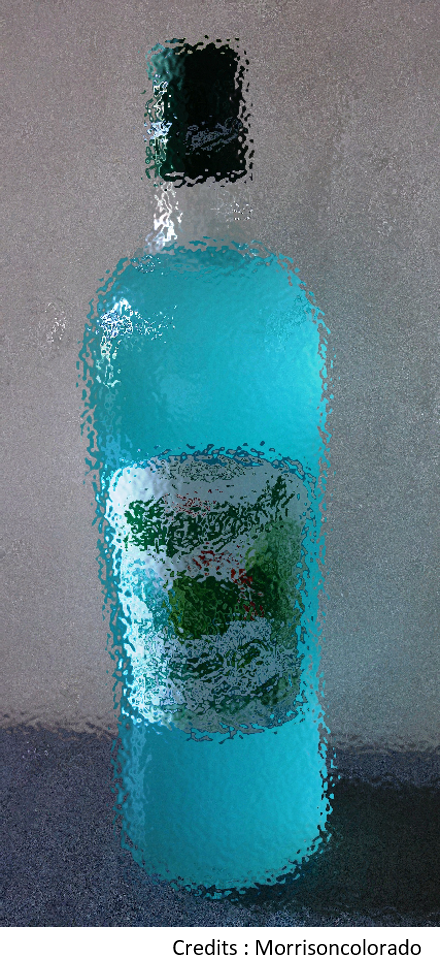
\includegraphics[scale=0.35]{Images/Sirop_menthe.png}
  \end{wrapfigure}
Certains sirops de menthe de couleur bleue utilise un colorant alimentaire appelé E131. \textbf{On cherche à déterminer la concentration en masse de ce colorant}, qu'on notera $C_{m,com}$, d'un sirop de menthe commercial à l'aide d'un dosage.\\
Pour cela, on réalise \textbf{une échelle de teintes} constituées de quatre solutions fille étalons notées S$_1$, S$_2$, S$_3$ et S$_4$, de volume $V_{f}=20,0$~mL, obtenues après dilution d'une solution mère de concentration en masse de colorant E131 $C_{m,m}=12,0$~mg.L$^{-1}$. On note $V_{m}$ le volume de solution mère prélevé pour obtenir les solutions filles.\\
\begin{tabular}{|C{0.6}|C{0.13}|C{0.13}|C{0.13}|C{0.13}|}
    \hline
    \cellcolor{orange!25} Solution fille & S$_1$ & S$_2$ & S$_3$ & S$_4$ \\
    \hline
    \cellcolor{orange!25} V$_m$ (en mL) & 13,3 & 10,0 &  & 2,5 \\
    \hline 
    \cellcolor{orange!25} V$_f$ (en mL) & 20,0 & 20,0 & 20,0 & 20,0 \\
    \hline
    \cellcolor{orange!25} Facteur de dilution F & 1,5 & 2,0 & & 8,0 \\
    \hline
    \cellcolor{orange!25} Concentration en masse solution fille $C_{m,f}$ (en mg.L$^{-1}$) & 8,0 & 6,0 & 3,0 & 1,5 \\
    \hline
\end{tabular}
\\

\question{En détaillant les calculs, compléter le tableau de l'énoncé. (3pts) }{
\begin{equation*}
    F = \frac{C_{m,m}}{C_{m,f}} ~(1pt)~= \frac{12,0}{3,0} = 4,0 ~(0,5+0,5=1pt)
\end{equation*}
On en déduit le volume $V_m$ :
\begin{equation*}
    V_m = \frac{V_f}{F}~(1pt) = \frac{20,0}{4,0} = 5,0~(0,5+0,5=1pt)
\end{equation*}
Voici le tableau complété (0,5pt):\\
\begin{tabular}{|C{0.35}|C{0.13}|C{0.13}|C{0.13}|C{0.13}|}
    \hline
    \cellcolor{orange!25} Solution fille & S$_1$ & S$_2$ & S$_3$ & S$_4$ \\
    \hline
    \cellcolor{orange!25} V$_m$ (en mL) & 13,3 & 10,0 & \textcolor{red}{5,0} & 2,5 \\
    \hline 
    \cellcolor{orange!25} V$_f$ (en mL) & 20,0 & 20,0 & 20,0 & 20,0 \\
    \hline
    \cellcolor{orange!25} Facteur de dilution F & 1,5 & 2,0 & \textcolor{red}{4,0} & 8,0 \\
    \hline
    \cellcolor{orange!25} Concentration en masse solution fille $C_{m,f}$ (en mg.L$^{-1}$) & 8,0 & 6,0 & 3,0 & 1,5 \\
    \hline
\end{tabular}}{0}
\\
\vspace{-5pt}
\question{Le sirop de menthe est dilué 10 fois. La teinte du sirop de menthe dilué est comprise entre celle des solutions S$_1$ et S$_2$. Déterminer un encadrement de la concentration en masse de la solution de menthe dilué. (1pt)}{\begin{equation*}
    6,0~\text{mg.L$^{-1}$} < C_{m,\text{sirop dilué} }< 8,0~\text{mg.L$^{-1}$}
\end{equation*}}{0}
\\
\vspace{-5pt}
\question{En déduire un encadrement de $C_{m,com}$. (1pt)}{Comme on a dilué 10 fois, les valeurs de l'encadrement précédent doivent être multipliées par 10 ce qui donne :
\begin{equation*}
    60~\text{mg.L$^{-1}$} < C_{m,com} < 80~\text{mg.L$^{-1}$}
\end{equation*}}{0}
\\
\vspace{-5pt}
\question{Choisir la verrerie pour diluer le sirop de menthe. \textbf{Vous ferez attention à donner des valeurs correctes des volumes de chaque verrerie utilisée.} (2,5pts)}{Verrerie pour une dilution par 10 de la solution mère : un bécher pour contenir le sirop (0,5pt), une pipette jaugée de 10,0 mL pour prélever le sirop dans le bécher (0,5+0,5=1pt), une
fiole jaugée de 100,0 mL pour avoir un facteur de dilution de 10 ($V_{\text{fiole}}=10\times V_{\text{prélevé}}$) (0,5+0,5=1pt)}{0}
\\
\vspace{-5pt}
\question{Proposer une méthode pour diminuer l'incertitude sur la concentration en masse de la solution commerciale (1pt).}{On pourrait réaliser plus de solutions filles dont les concentrations seraient comprises entre 6,0 mg.L$^{-1}$ et 8,0 mg.L$^{-1}$.\\
On peut également réaliser une courbe d'étalonnage en mesurant la masse volumique de solutions contenant du colorant E131 en fonction de leur concentration en masse de ce colorant puis mesurer la masse volumique du sirop (préalablement dilué) et en déduire sa concentration en masse par lecture graphique.}{0}
\end{doc}

%\begin{center}
 %   \includegraphics[scale=0.85]{Images/Feuilles/Grands_carreaux.pdf}
%\end{center}


\end{document}